\documentclass[12pt]{article}

\usepackage{sbc-template}

\usepackage{graphicx,url}

\usepackage[brazil]{babel}
%\usepackage[latin1]{inputenc}
\usepackage[utf8]{inputenc}
\usepackage[T1]{fontenc}
\usepackage{ae}

%%-----------------------------------------------------------
%% Pacotes para incluir código-fonte
\usepackage{listings}

\lstset{numbers=left,
stepnumber=1,
firstnumber=1,
numberstyle=\tiny,
extendedchars=true,
breaklines=true,
frame=tb,
basicstyle=\footnotesize,
stringstyle=\ttfamily,
showstringspaces=false
}
\renewcommand{\lstlistingname}{Código}
\renewcommand{\lstlistlistingname}{Lista de Listagens}
%%----------------------------------------------------------

\sloppy

%%%%-------------------------------------------------------------%%%%
%%%%                INFORMAÇÕES GERAIS                           %%%%
%%%%-------------------------------------------------------------%%%%

\author{Darlisson Marinho de Jesus\inst{1}, Raimundo Correa Oliveira}

\address{
  Universidade do Estado do Amazonas -- UEA\\
  Av. Darcy Vargas, 1200, Parque 10 de Novembro -- 69.065.020 -- Manaus --
  AM -- Brasil \\
  \email{\{darlisson11, rcorrea.oliveira\}@gmail.com} %%, \{dmdj.eng\}@uea.edu.br}
}
%%----------------------------------------------------------




\usepackage{subfigure}
\usepackage{titlesec}
%\setcounter{secnumdepth}{4}
%\titleformat{\paragraph}
%{\normalfont\normalsize\bfseries}{\theparagraph}{1em}{}
%\titlespacing*{\paragraph}
%{0pt}{3.25ex plus 1ex minus .2ex}{1.5ex plus .2ex}
\usepackage[hidelinks]{hyperref}
\usepackage{amsmath}
\usepackage{xcolor}         % Pacote de cores
 
% Define cores em RGB
\definecolor{dkgreen}{rgb}{0,0.6,0}
\definecolor{gray}{rgb}{0.5,0.5,0.5}
\definecolor{mauve}{rgb}{0.58,0,0.82}
 
% Configuração para exibir código e C++
\lstset{
language = C, % Linguagem de programação
basicstyle = \footnotesize, % Tamanho da fonte do código
numbers = left, % Posição da numeração das linhas
numberstyle = \tiny\color{blue}, % Estilo da numeração de linhas
stepnumber = 1, % Numeração das linhas ocorre a cada quantas linhas?
numbersep = 10pt, % Distância entre a numeração das linhas e o código
backgroundcolor = \color{white}, % Cor de fundo
showspaces = false, % Exibe espaços com um sublinhado
showstringspaces = false, % Sublinha espaços em Strings
showtabs = false, % Exibe tabulação com um sublinhado
frame = trBL, % Envolve o código com uma moldura, pode ser single ou trBL
rulecolor = \color{black}, % Cor da moldura
tabsize = 2, % Configura tabulação em x espaços
captionpos = b, % Posição do título pode ser t (top) ou b (bottom)
breaklines = true, % Configura quebra de linha automática
breakatwhitespace= false, % Configura quebra de linha
title = \lstname, % Exibe o nome do arquivo incluido
%caption = \lstname, % Também é possível usar caption no lugar de title
keywordstyle = \color{blue}, % Estilo das palavras chaves
commentstyle = \color{dkgreen}, % Estilo dos Comentários
stringstyle = \color{mauve}, % Estilo de Strings
escapeinside = {\%*}{*)}, % Permite adicionar comandos LaTeX dentro do seu código
morekeywords ={float2} % Se quiser adicionar mais palavras-chave
}


\title{Análise Comparativa do Desempenho de Unidades de Processamento Gráfico Nvidia e ATI através de filtros digitais de imagens}

\begin{document}
\maketitle
\begin{abstract}
Graphics Processing Unit (GPU) are high performance co-processors intendend, originally, to improve the use and quality of computer graphics applications.  However, the GPU aplications has been extended to other fields to general purpose, such as digital image processing. In this study, we compared the performance of some models of GPU from Nvidia and ATI manufacturers, through the implementation of the  Sobel filter to edge detection and  lowpass filter with the OpenCL language. The digital filters implemented in the models GPU of Nvidia, presented the best run time and data transfer rates of memory.

\end{abstract}
\begin{resumo}
Unidades de processamento gráfico ou GPU  (do inglês,  \textit{Graphics Processing Unit})  são co-processadores de alto desempenho destinados inicialmente a melhorar ou prover de capacidade gráfica a um computador. Porém, as aplicações para GPUs tem sido expandida à outras áreas para fins gerais, como o processamento digital de imagens. Neste trabalho, foi comparado o desempenho da de alguns modelos de GPU dos fabricantes Nvidia e ATI, através da implementação do filtro de detecção de borda Sobel e o filtro Passa-baixa na linguagem OpenCL (do inglês, \textit{Open Computing Language}). Os filtros digitais executados nos modelos de GPU da Nvidia apresentaram os melhores de tempo de execução e taxas de transferência de dados da memória.
\end{resumo}

\section{Introdução}
%\section{Descrição do Problema}
Segundo Zhang, \cite{ArchComp}, nos últimos anos, modernas unidades de processamento gráfico têm sido amplamente adotadas em áreas de computação de alto desempenho para resolver problemas de cálculo em grande escala.  
Tais problemas são encontrados na área de processamento de digital de imagem, onde muitos algoritmos são computacionalmente caros, mas paralelizáveis \cite{Gonzalez:2006:DIP:1076432}. Além disso, os métodos tradicionais de processamento não conseguem satisfazer a exigência de tempo real para o processamento de imagem com grandes dimensões. Uma possibilidade para otimizar esse tempo é utilizar a programação para GPU, denominado GPGPU (do inglês, \textit{General Purpose Graphics Processing Unit}). No trabalho de Nan Zhang, \cite{ImgParallel}, os resultados mostraram que algoritmos paralelos para o processamento de imagens implementados em GPU, podem alcançar notável aumento de velocidade, em comparação com métodos sequenciais baseados na CPU (do inglês, \textit{Central  Processing  Unit}). 

Além disso, como resultado da recente evolução dos processadores gráficos e ferramentas para sua programação, pesquisadores, cientistas e desenvolvedores, tornaram-se os maiores interessados em usufruir  do poder destes processadores, principalmente no contexto da computação científica. Contudo, surge a necessidade de comparar o desempenho computacional das GPUs dos diferentes fabricantes. Uma vez que, tais informações podem auxiliar engenheiros e cientistas na busca do melhor desempenho de suas soluções, aliado ao menor custo das tecnologias com o passar do tempo. A Nvidia e a ATI, são as duas principais fabricantes das GPUs modernas. Essas empresas desenvolvem também, as tecnologias utilizadas  para  atender a demanda de desenvolvimento de aplicações de propósito geral com as GPUs. 

A primeira, o CUDA (do inglês, \textit{Compute Unified Device Architecture}) \cite{NvidiaCuda}, foi desenvolvida pela pioneira NVIDIA e permite aumentos significativos de performance computacional ao aproveitar a potência da unidade de processamento gráfico (GPU). Mas, apesar de ser a tecnologia mais utilizada no mercado, ela é restrita para as placas gráficas fabricadas pela Nvidia, não permitido a portabilidade das aplicações para GPUs de outros fabricantes.

A outra tecnologia é o OpenCL \cite{opencl08}, que é um padrão aberto para programação paralela de propósito geral em CPUs, GPUs e outros processadores. Ele consiste de uma API para coordenar computação paralela entre processadores heterogêneos e uma linguagem de programação multi-plataforma baseada na C99.  O OpenCL é gerido pelo consórcio tecnológico Khronos Group e  entre os desenvolvedores estão a Intel, IBM, Apple, AMD, Nvidia etc. A  portabilidade da aplicação é um dos requisitos obrigatórios para que possamos  comparar o desempenho  de  GPUs de diferentes fabricantes, por isso, usaremos  o OpenCL como recurso para implementar o filtro detector de bordas Sobel e o filtro Passa-baixa, pois com o OpenCL é  possível escrever programas para dispositivos diferentes. O principal objetivo deste trabalho é comparar o desempenho das Unidades de Processamento Gráfico das fabricantes NVIDIA e ATI, através do Processamento Digital de Imagens com os filtros Passa-baixa e o filtro Sobel para detecção de borda implementados na linguagem OpenCL. Assim, identificaremos a GPU que apresenta o melhor desempenho quando se utiliza  a linguagem OpenCL como recurso computacional. 

Nosso trabalho faz contribuições interessantes, pois até o presente momento não encontramos registros de trabalhos que fazem uma análise comparativa do desempenho das placas gráficas da Nvidia e ATI, usando filtros para o processamento digital de imagens, escritos com o OpenCL. Além disso, este trabalho contém implementações de filtros digitais para imagens em GPU usando o OpenCL.

Este trabalho está organizado nas seguites seções: \textit{Trabalhos Relacionados}, onde apresentamos os trabalhos que estão relacionados ao nosso, enfatizando os resultados e metodologia de cada um. Na seção \textit{Arquitetura de uma GPU}, fazemos uma breve descrição da arquitetura de uma GPU moderna, apresentamos as diferenças de projetos entre uma CPU e  apresentamos as arquiteturas das GPUs utilizadas neste trabalho. A linguagem OpenCL é descrita na seção \textit{OpenCL}, onde explicamos o seu propósito como uma linguagem para programação paralela. A definição do filtro Sobel e o filtro Passa-baixa, implementados neste trabalho, é feita na seção \textit{Aplicações}. Na seção \textit{Metodologia} é apresentada os métodos utilizados para atingir nossos resultados, assim como, as ferramentas para isso. Por fim, na seção \textit{Resultados e Discussões} apresentamos os resultados alcançados neste trabalho.

\section{Trabalhos Relacionados}
Purcell \cite{Purcell:2002:RTP:566654.566640} foi quem realizou as primeiras experiências envolvendo GPUs programáveis. Seu trabalho demonstrou que o algoritmo (um algoritmo de  ray tracing)  escrito em  assembly  para a  NVIDIA GeForce 3,  no processador de fragmentos, conseguia ter um desempenho maior em GPU do que na CPU. Este trabalho publicado nos primórdios da era GPGPU (do inglês, \textit{General Purpose Graphics Processing Unit}) demonstrou o  potencial do hardware gráfico programável como um dispositivo para computação genérica e paralela. 

Uma comparação do desempenho do CUDA em contraste com o OpenCL foi feita por Kamrin \cite{CudaOpenCl}, através da implementação de uma aplicação científica com elevado custo computacional, simulação Monte Carlo de um sistema de spin, para  medir e compararem o tempo de transferência de dados da GPU para a CPU e viceversa. Os tempos de execução dos  kernels e os tempos de execução do ciclo de vida completo das execuções, tanto para o CUDA quanto para o OpenCL. Neste trabalho os testes restringiram-se a uma GPU da própria Nvidia e os autores concluíram que o CUDA era a melhor escolha para aplicações de alta performance. 

Em \cite{SIMD}, os autores propuseram algoritmos eficientes para  o  processamento  linear  de imagem, explorando as extensões SIMD (do inglês, \textit{Single Instruction, Multiple Data}) fornecidas em processadores AMD e Intel.  O trabalho experimental e os resultados obtidos sugeriram  que  implementações baseadas em OpenCL proporcionaram um rendimento mais baixo, uma média de 1,8 vezes, do que implementações equivalentes que utilizam diretamente o SIMD intrínsecos suportado pelo compilador Intel. 
O interessante neste trabalho é a aplicação heterogênea que se pode fazer com o OpenCL, que pode ser usado tanto para GPUs quanto para processadores multi-cores. 

Uma comparação entre CPU e GPU com o filtro de detecção de borda Sobel foi feita por Zhang \cite{ImgParallel}, onde os resultados experimentais indicaram que otimizações no tempo de transferência de dados entre a memória do computador e a memória da placa gráfica, podem melhorar em até 25 vezes o desempenho da implementação desse filtro para GPU.
\section{Arquitetura de uma GPU}
As GPUs são compostas de centenas de núcleos escalares, (cores), que executam o mesmo código através de centenas a milhares de threads concorrentes. Esta abordagem se opõe ao modelo tradicional de processadores multicore, onde algumas unidades de núcleos completos e independentes são capazes de processar threads ou processos. Estes núcleos completos, as CPUs, possuem poderosas unidades de controle e de execução capazes de executar instruções paralelas e fora de ordem, além de contarem com uma poderosa hierarquia de cache. Já as GPUs contam com unidades de controle e de execução mais simples, onde uma unidade de despacho envia apenas uma instrução para um conjunto de núcleos que a executarão em ordem. 

Na Figura \ref{fig:cpu_gpu}, podemos observar as diferenças entre as filosofias de projeto fundamentais nos dois tipos de processadores. Segundo David Kirk, \cite{programando}, a arquitetura da CPU é otimizada para o desempenho de código sequencial. Ela utiliza uma lógica sofisticada para permitir que instruções de uma única thread de execução sejam executadas em paralelo ou mesmo fora de sua ordem sequencial. Enquanto que, a filosofia de projeto das GPUs é modelada pela crescente indústria de videogames que exerce uma tremenda pressão econômica para a capacidade de realizar um número maciço de cálculos de ponto flutuante por quadro. A solução que prevalece até o momento é otimizar para a vazão de execução do número maciço de threads. Outra característica importante é a hierarquia de memória. As GPUs, possuem memória global que pode ser acessada por todas as threads, porém as mais modernas já contam com caches de nível 1 e de nível 2. Além disso, outras memórias especializadas também podem ser usadas para acelerar o processamento.

\FloatBarrier
\begin{figure}[!ht]
\centering
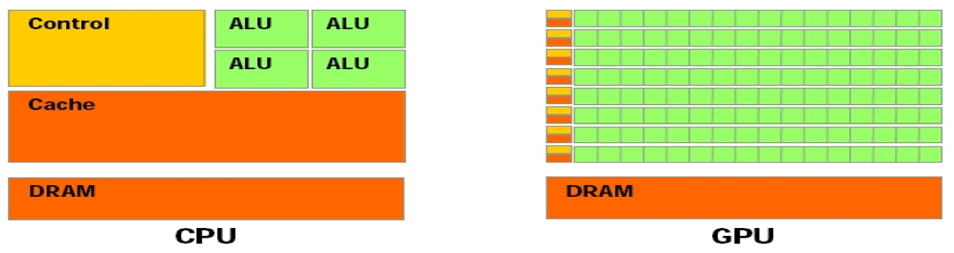
\includegraphics[width=14cm]{cpu_gpu.png}
\caption{CPUs e GPUs têm filosofias de projeto fundamentalmente diferentes. Fonte: \cite{programando}.}
\label{fig:cpu_gpu}
\end{figure}
\FloatBarrier
\subsection{Arquitetura Nvidia Tesla}
A arquitetura Nvidia Tesla baseia-se em uma matriz de processadores escaláveis. A Figura  \ref{fig:tesla} mostra um diagrama de blocos da GPU GeForce 8800, GPU que introduziu a arquitetura Tesla em novembro de 2006, com 128 \textit{stream processors} (SP) organizados em 16 multiprocessadores de stream (SMs), em oito unidades de processamento independentes chamado TPCs (\textit{texture/processors cluster}). Cada SP tem uma unidade de multiplicação-adicção (MAD) e uma unidade de multiplicação. Com os 128 SPS, têm-se um total de 500  gigaflops. 
Cada GPU atualmente possui memória do tipo DRAM GDDR (\textit{Graphics Double Data Rate}), chamado \textit{memória global} na Figura \ref{fig:tesla}. Essas DRAMs GDDR diferem das DRAMs do sistema na placa-mãe da CPU porque são basicamente a memória do frame buffer que é usada para os gráficos.  A arquitetura Tesla foi a primeira plataforma de supercomputação onipresente. A NVIDIA vendeu mais de 50 milhões de GPUs baseados em Tesla. 

A GPU Nvidia GeForce 210 foi construída com essa arquitetura e é usada neste trabalho. Ela possui 2 multiprocessadores de streamming com 8 SP cada, totalizando 16 processadores de streaming.


\FloatBarrier
\begin{figure}[!ht]
\centering
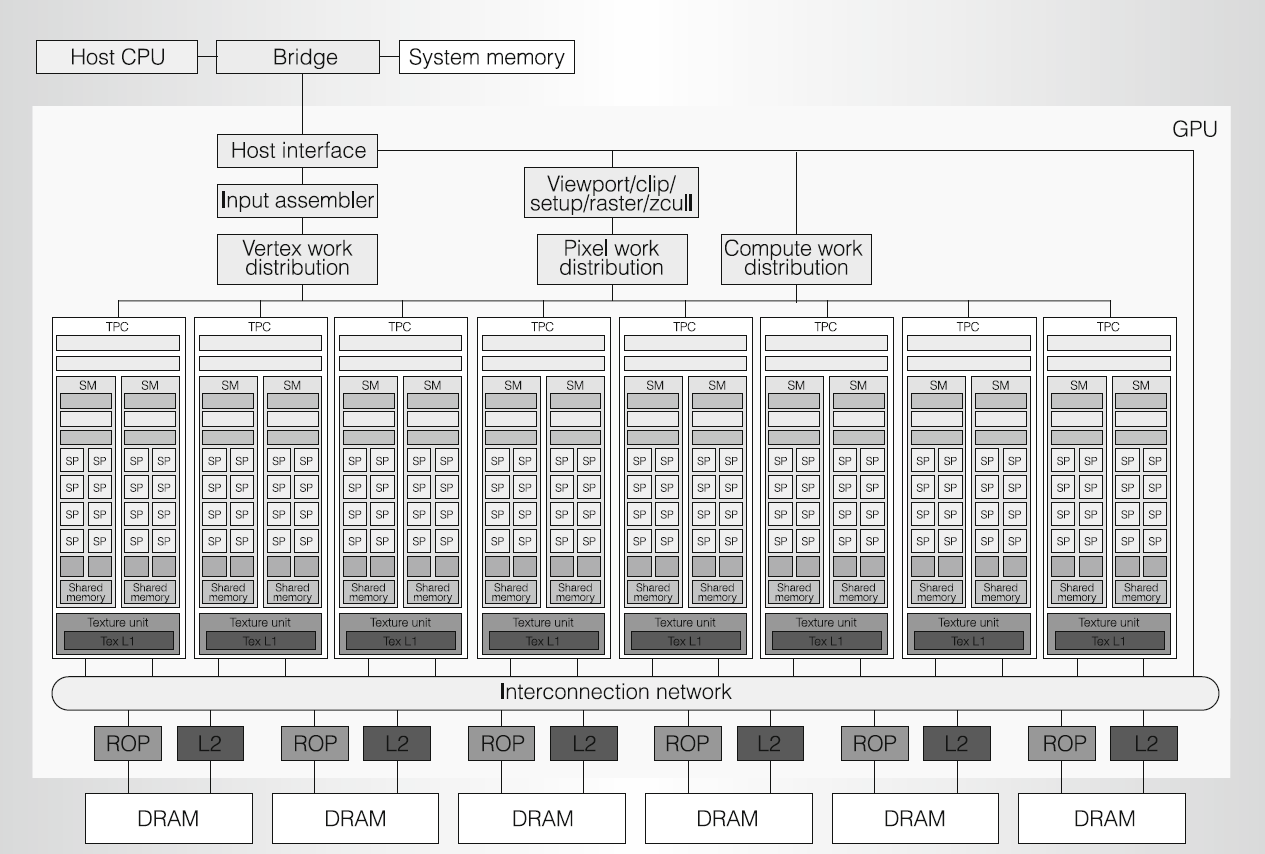
\includegraphics[width=12cm]{tesla.png}
\caption{Arquitetura Nvidia Tesla. TPC:texture/processor cluster; SM: streaming multiprocessor; SP: stream processor; Tex: texture, ROP: raster operation processor. Fonte:(\cite{NvidiaTesla})}
\label{fig:tesla}
\end{figure}
\FloatBarrier
\subsection{Arquitetura Nvidia Fermi}
Lançada em abril de 2010, esta arquitetura trouxe suporte para novas instruções para programas em C++, como alocação  dinâmica de objeto e tratamento de exceções em operações de try e catch. Cada SM de um processador Fermi possui 32 CUDA cores. Até 16 operações  de precisão dupla por SM podem ser executadas em cada ciclo de clock \cite{NvidiaFermi}.
Além disso, cada SM possui:
\begin{itemize}
\item  Dezesseis unidades de load e store, possibilitando que o endereço de fonte e destino possam ser calculados
para dezesseis threads por clock. \\
\item Quatro Special Function Units (SFUs), que executam instruções  transcendentais, como seno, cosseno, raiz
quadrada, etc. Cada SFU executa uma instruções  por thread por ciclo. O pipeline da SFU é desacoplado
da dispatch unit, permitindo que esta possa realizar o issue (despacho) de outra instrução enquanto a SFU
está ocupada.
\end{itemize}
A Figura \ref{fig:fermi} apresenta a visão geral da arquitetura Fermi. A GPU Nvidia GeForce GT 520, que é usada neste trabalho, é fabricada com a segunda geração dessa arquitetura e ela possui um total de 48 processadores de streammimg em um único multiprocessador de streaming SM.  
\begin{figure}[!ht]
\centering
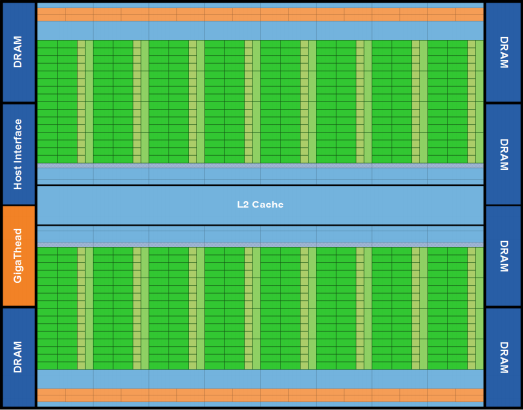
\includegraphics[width=10cm]{fermi_2.png}
\caption{Visão geral da arquitetura Nvidia Fermi}
\label{fig:fermi}
\end{figure}
\FloatBarrier
\subsection{Arquitetura ATI Caicos}
De codinome Caicos, esta arquitetura foi lançada em 7 de fevereiro de 2011 com um único produto, a GPU Radeon HD 6450.
A GPU ATI Radeon HD 6450, foi usada neste trabalho, ela possui 160 \textit{stream cores} e 2 mecanismos SIMDs (parecido com os multiprocessadores de streaming (SM) da Nvidia), cada um com 80 stream core. Os streams cores usam a tecnologia VLIW (do inglês, \textit{Very Long Instruction Word}), o que permite a execução de um grupo de instruções ao mesmo tempo.
\FloatBarrier
\begin{figure}[!ht]
\centering
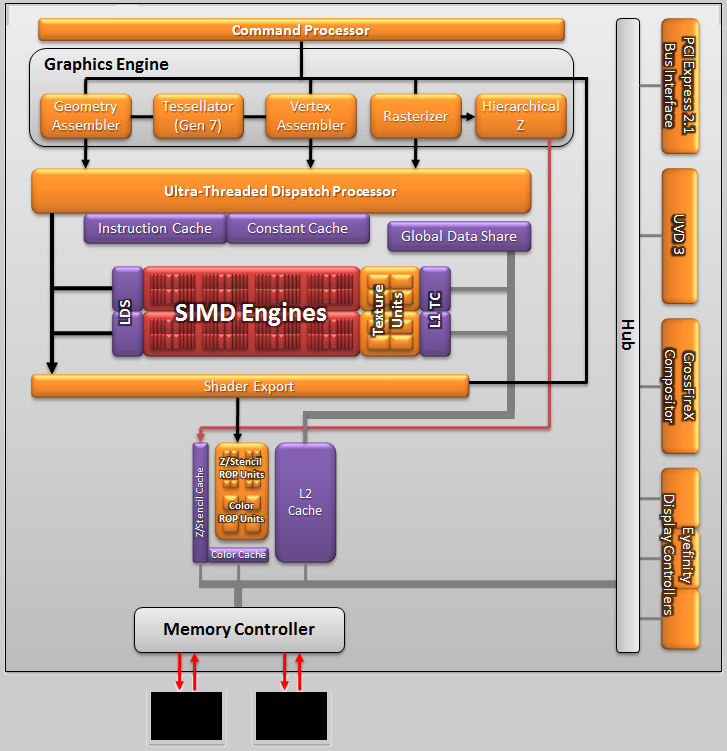
\includegraphics[width=10cm]{caicos.jpg}
\caption{Visão geral da arquitetura ATI Caicos}
\label{fig:caicos}
\end{figure}
\FloatBarrier
\section{OpenCL}
A linguagem OpenCL é uma API (do inglês, \textit{Application Programming  Interface})  padrão  para  programação  de  computadores  compostos  de  uma  combinação  de  CPUs,  GPUs e  outros processadores. Estruturas como essas são conhecidas como sistemas  heterogêneos. O OpenCL é um padrão aberto mantido pelo Khronos group e voltado para o desenvolvimento paralelo em sistemas heterogêneos contendo CPUs, GPUs e outros aceleradores \cite{opencl08}. O OpenCL é baseada em um subconjunto estendido do padrão ISO C99 e, portanto, é muitas vezes referido como  OpenCL C. 

O modelo de execução proposto pelo OpenCL se baseia em dispositivos contendo diversas unidades computacionais ( \textit{compute unit}) capazes de gerenciar grupos de threads chamados\textit{workgroups}. Esses grupos de threads executam uma mesma rotina, chamada de \textit{Kernel}, sobre dados diferentes, sendo um modelo de programação totalmente compatível com implementações paralelas de algoritmos para o processamento de imagens. Ao contrário de CPUs que contam com uma hierarquia multinível de cache, algumas GPUs possuem apenas uma cache de instruções e uma memória local de baixa latência compartilhada entre elementos do workgroup, que deve ser explicitamente manipulada pelo algoritmo. Por ser um framework aberto e padronizado, independente de fabricante, o OpenCL aparece como uma alternativa conveniente para sistemas computacionais que demandem desempenho e portabilidade. 

Uma plataforma OpenCL é composta por um ou vários dispositivos computacionais ou (\textit{Devices}. Um \textit{device} pode ser uma GPU, por exemplo. Cada \textit{device} possui diversas unidades computacionais (\textit{comput units}), que possuem diversos elementos de processamento (\textit{processing elements})(ALU, cache, memória compartilhada). Já um \textit{kernel} é um programa escrito na linguagem OpenCL que é executado por todas as unidades computacionais ao mesmo tempo, que trata o fluxo de dados multiprocessado no modelo SIMD (do inglês, \textit{Single Instruction, Multiple Data}). O sistema computacional responsável pela agregação, inicialização e submissão de tarefas a diferentes devices OpenCL é denominado de \textit{Host}. \textit{Host}, \textit{devices}, \textit{compute units} e \textit{processing elements} compõem o modelo de plataforma da arquitetura OpenCL, como mostrado na Figura \ref{fig:opencl}.
\FloatBarrier
\begin{figure}[!ht]
\centering
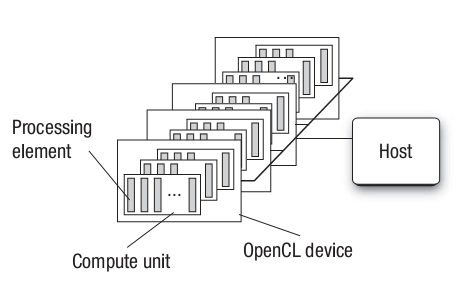
\includegraphics[width=10cm]{opencl.png}
\caption{O modelo de plataforma OpenCL com um host e um ou mais dispositivos OpenCL. Cada dispositivo OpenCL tem uma ou mais unidades de cálculo, cada um dos quais tem um ou mais elementos de processamento \cite{munshi2011opencl}}
\label{fig:opencl}
\end{figure}
\section{Aplicações}
\subsection{Filtro Sobel para detecção de borda}
\label{sec:sobel}
O filtro Sobel é uma operação utilizada em processamento de imagem, aplicada sobretudo em algoritmos de detecção de borda, e foi proposto por Irwin Sobel em \cite{Sobel:1970:CMM:905376}. Em termos técnicos, consiste num operador que calcula diferenças finitas, dando uma aproximação do gradiente da intensidade dos pixels da imagem. O filtro Sobel calcula o gradiente da intensidade da imagem em cada ponto, dando a direcção da maior variação de claro para escuro e a quantidade de variação nessa direcção. Assim, obtém-se uma noção de como varia a luminosidade em cada ponto, de forma mais suave ou abrupta. Com isto consegue-se estimar a presença de uma transição claro-escuro e de qual a orientação desta. Como as variações claro-escuro intensas correspondem a fronteiras bem definidas entre objectos, consegue-se fazer a detecção de borda \cite{Gonzalez:2006:DIP:1076432}.

Matematicamente este operador utiliza duas matrizes 3x3 que são convoluídas com a imagem original para calcular aproximações das derivadas - uma para as variações horizontais $Gx$ e uma para as verticais $Gy$. Sendo $A$ a imagem inicial então, $Gx$  e $Gy$  serão duas imagens que em cada ponto contêm uma aproximação às derivadas horizontal e vertical de $A$.
$$
Gx=\left[\begin{array}{rrr}
-1&0&+1\\
-2&0&+2 \\
-1&0&+1
\end{array}\right]*A\quad
Gy=\left[\begin{array}{ccc}
-1&-2&-1\\
 0& 0& 0 \\
+1&+2&+1
\end{array}\right]*A
$$

A magnitude do gradiente é dado por:

$$
|G|=\sqrt{Gx^2 + Gy^2}
$$

O código fonte em OpenCL encontra-se no Apêndice \textbf{A}.
\subsection{Filtro Passa-baixa}
\label{sec:passa_baixa}
Um filtro do tipo passa-baixa deixa passar as baixas frequências e elimina os valores relacionados às altas frequências. Portanto, o efeito deste filtro é o de suavizar a imagem, uma vez que as altas frequências que correspondem às transições abruptas são atenuadas. A suavização tende pelo mesmo motivo, diminuir o ruído em imagens.
\cite{Gonzalez:2006:DIP:1076432}

Neste trabalho foi implementado o filtro passa-baixa ideal que opera no domínio da frequência. E para isso, foi necessário implementar o algoritmo que computa a Transformada Rápida de Fourier, uma vez que a idéia básica dos filtros no domínio da frequência está em computar a Tranformada de Fourier da imagem a ser filtrada, multiplicar este resultado pela função de transferência do filtro e extrair a Inversa da Transformada de Fourier do resultado  

De acordo com Vieira, \cite{MarquesFilho1999}, sendo $F(u,v)$ a transformada de Fourier da imagem a ser processada e sendo $G(u,v)$ a transformada de Fourier da imagem que se deseja obter à saída (com os componentes de alta frequência atenuados), a filtragem passa-baixas consiste em encontrar um $H(u,v)$ tal que: 
$G(u,v) = F(u,v)H(u,v)$

\paragraph{Filtro passa-baixas ideal} - Segundo \cite{Gonzalez:2006:DIP:1076432}, um filtro passa-baixas 2-D ideal é aquele cuja função de transferência satisfaz a relação:
$$
H(u,v)=\begin{cases}
1,	&\mbox{se}\quad D(u,v)\le Do,\\
0,	&\mbox{se}\quad D(u,v)x>Do.
\end{cases}
$$

onde $Do$ é um valor constante positivo e $D(u,v)$ é a distância do ponto $(u,v)$ à origem do plano de frequência, que é obtido por: 

$$
D(u,v) = \sqrt{(u - P/2)^2 + (v - Q/2)^2}
$$

onde, $P$ e $Q$ são, respectivamente, a largura e a altura da imagem. Quanto menor o raio $Do$, menor a frequência de corte e, portanto, maior o grau de borramento da imagem resultante. 
Em nosso trabalho definimos $Do$ como sendo $Do=DimensãoDaImagem/8$, esse valor foi o que melhor se encaixou em nossos testes.
O código fonte em OpenCL encontra-se no Apêndice \textbf{A}.

\section{Objetivo Geral}
Comparar o desempenho das Unidades de Processamento Gráfico das fabricantes NVIDIA e ATI, através do Processamento Digital de Imagens com os filtros Passa-baixa e o filtro Sobel para detecção de borda implementados na linguagem OpenCL. Assim, identificaremos qual GPU apresenta o melhor desempenho quando se utiliza  a linguagem OpenCL como recurso computacional para a implementação destes filtros.
\subsection{Objetivos Específicos}
\begin{itemize}
\item Determinar os indicadores de desempenho que permitam avaliar as rotinas destes filtros no contexto das Unidades de Processamento Gráfico;\\

\item Avaliar a arquitetura das GPUs da Nvidia e ATI, buscando identificar as diferenças que podem afetar no desempenho das implementações;\\

\item Implementar o algoritmo do filtro Passa-baixa na linguagem OpenCL e obter os dados de desempenho das GPUs Nvidia e ATI;\\

\item Implementar o algoritmo do filtro para detecção de borda Sobel na linguagem OpenCL e obter dados de desempenho das GPU Nvidia e ATI;\\
\end{itemize}
%%-----------------------------------------------------------------------------
%% Metodologia
\section{Metodologia}
Nesta seção será apresentada a metodologia adotada nesse trabalho para obter os resultados finais, isto é, o resultado da avaliação de desempenho das Unidades de Processamento Gráfico Nvidia e ATI.
\subsection{Métodos}
A pesquisa, quanto aos objetivos, conduz a uma experimentação, desta forma, caracterizando-se como pesquisa experimental, assim, foi realizado um estudo da especificação do OpenCL 1.1 \cite{opencl08} e dos principais conceitos de filtragem digital, tanto no domínio do tempo, quanto no domínio da frequência. Os filtros implementados neste trabalho, o filtro Passa-baixa, o filtro Sobel para detecção de borda e a rotina da Transformada Rápida de Fourier, foram embassados no livro do Rafael Gonzalez \cite{Gonzalez:2006:DIP:1076432}.

A etapa seguinte, consistiu em montar o hardware necessário, sobre o qual foram realizados os testes de desempenho. Foram utilizados 3 computadores, com as mesmas configurações de processador, memória, placa-mãe, etc; e cada um, desses computadores, foi equipado com as placas gráficas: Nvidia Geforce GT 520, Nvidia Geforce 210 e ATI Radeon HD 6450. As aplicações foram implementados na linguagem C e OpenCL, com o Microsoft Visual Studio 2010 professional e o kit de desenvolvimento disponibilizadas por cada um dos fabricantes das placas.
\subsubsection{Dados de entrada}
Nossos dados de entrada consistiram de um total de 32 imagens no formato \textit{PGM} ( do inglês, \textit{Portable Gray Map}), divididas em 8 amostras para cada uma das seguintes dimensões (em pixels): 256x256, 512x512, 1024x1024 e 2048x2048. Estas imagens foram obtidas no banco de dados de imagens proposto em \cite{MartinFTM01}. E teve como objetivo avaliar o desempenho das GPUs com os filtros propostos na seção \textbf{\ref{sec:sobel}} e \textbf{\ref{sec:passa_baixa}}, sob o ponto de vista do tempo médio de execução do \textit{kernel}(programa executado exclusivamente pela GPU) e as taxas média de transferências da memória, tanto da memória do Host para a memória do device quanto da memória do device para a memória do Host.
\subsubsection{Coleta dos dados}
\label{coleta}
A coleta de dados consistiu em submeter as amostras aos Filtros Sobel e Passa-baixa, em cada uma das placas gráfica utilizadas neste trabalho e coletar essas métricas com as ferramentas descritas abaixo:
\paragraph{Nvidia Nsight 3.0} -  De acordo com o manual \cite{NvidiaNsight}, trata-se de um ambiente de desenvolvimento para aplicações CUDA e aplicações gráficas que são executadas em GPUs da NVIDIA. O Nvidia Nsight 3.0, permite também, a depuração e análise de desempenho da aplicações escritas em OpenCL.

Os dados coletados para este trabalho, foram obtidos a partir de relatórios gerados manualmente, no formato CSV (do inglês, \textit{Comma Separated Values}), uma vez que o Nvidia Nsight somente gera relatórios automáticos em um formato proprietário que somente podem ser lidos com Visual Studio. O Nvidia Nsight está na versão 3.0 e está disponível para o Windows como uma extensão para o Visual Studio no Windows e para o Linux, como um plugin para o Eclipse IDE.

\paragraph{AMD CodeXL 1.2} - O manual do AMD CodeXL, o descreve como um conjunto de ferramentas que permite aos desenvolvedores aproveitarem os benefícios das CPUs, GPUs e APUs (do inglês, \textit{Accelerated processing unit}) da AMD, ajudando-os a identificar erros de programação e problemas de desempenho em sua aplicação de forma rápida e fácil. Permite aos desenvolvedores, depurar, realizar profile e análise estática dos códigos de suas aplicações sobre GPU,CPU e APU da AMD.

Neste trabalho, o profiler de GPU foi a principal funcionalidade usada. Esse profiler coleta e exporta automaticamente os dados de desempenho da aplicação OpenCL para relatórios em HTML (do inglês, \textit{HyperText Markup Language}). Apenas os relatórios de tempo de execução e taxas de transferência da memória foram analisados. O AMD CodeXL está na versão 1.2 e está disponível como uma extensão para o Visual Studio e como um aplicativo com interface de usuário para Windows e Linux. O manual é disponibilizado por \cite{AMDCodeXL}.
\subsubsection{Análise dos dados}
O formato dos relatórios gerados pelas ferramentas de profile dificultavam a recuperação e organização dos dados,  e devido a isso, foi desenvolvido uma ferramenta para automatizar a recuperação e consolidação desses dados. Os dados das métricas de desempenho, tempo de execução e taxas de transferência da memória, foram agrupados pela dimensão das amostras (256x256,512x512,1024x1024 e 2048x2048, em pixels), ou seja, foram 8 valores de tempo execução para as imagens de 256x256 pixels e assim por diante para as outras dimensões e métricas.
%\subsubsection{Tempo Médio de Execução do Kernel}
\paragraph{Tempo Médio de Execução do Kernel} - O tempo de execução do kernel da aplicação, corresponde ao tempo, em milisegundos, em que essa rotina permanence em execução pela GPU. No caso da aplicação do filtro Passa-baixa, que é formado por vários kernels, o tempo de execução corresponde a soma dos tempos de execução individual de cada kernel.

O tempo médio de execução foi calculado aplicando-se o cálculo da média aritmética sobre o conjunto de dados de tempo de execução, obtidos pelas ferramentas de profile e descritos na \textbf{secção \ref{coleta}}.
%\subsubsection{Taxa Média de Transferência Dados da Memória}
\paragraph{Taxa Média de Transferência Dados da Memória} - A taxa de transferência de dados corresponde ao número de bytes por unidade de tempo transmitidos entre a memória do computador e a memória da placa gráfica de forma bi-direcional. A amostra com o maior tamanho, possuía 4,194,344 bytes,  e a menor, 65,551 bytes.
A taxa média de transferência de dados da memória foi calculado aplicando-se o cálculo da média aritmética sobre o conjunto de dados de taxas de transferência, obtidos pelas ferramentas de profile descritas na \textbf{secção \ref{coleta}}. 
\FloatBarrier
\subsection{Materiais}
Os seguintes equipamentos foram utilizados para execução dos programas em nossos experimentos:
\begin{itemize}
\item Três PC/x64 com Sistema Operacional Microsoft Windows 7 Professional 64 Bits, Processador \textit{Intel\textregistered{} Core\texttrademark{} 2 Duo E7400} 2.80GHz e 4 GB de memória RAM.\\ 
\item Três Unidades de processamento gráfico. A Tabela \ref{tab:tab1} apresenta as especificações de hardware detalhados dessas GPUs.\newline

\end{itemize}
\begin{table}[!htb]
\begin{center}
\begin{tabular}{|l|c|c|c|}
%\hline
%\multicolumn{4}{|c|}{\textbf{Resumo das especificações das GPUs Nvidia e ATI }}\\
\hline
Modelo & \textbf{Geforce GT 520} & \textbf{Geforce 210} & \textbf{Radeon HD 6450}\\ 
\hline
Processadores de Stream & 48 & 16 & 160  \\ 
\hline
Clock do processador& 810 MHz & 589 MHz & 750 MHz \\ 
\hline
Arquitetura da GPU & Tesla & Fermi & Caicos\\ 
\hline
\textbf{Memória}& --- & --- & --- \\
\hline
Clock da memória & 900 MHz & 533 MHz & 1066 MHz \\ 
\hline
Tamanho da memória & 1024 MB & 512 MB & 1024 MB \\ 
\hline
Interface da memória & 64-bit & 64 -bit & 64-bit \\ 
\hline
Largura de Banda (GB/sec)& 14.4 & 8.0 & 8.5 \\ 
\hline
Tipo de memória	& DDR3 & DDR3 & DDR3 \\ 
\hline
\end{tabular}
\caption{Resumo das especificações das GPUs Nvidia e ATI}
\label{tab:tab1}
\end{center}
\end{table}
As seguintes ferramentas foram utilizadas para compilação dos programas:\newline

\begin{itemize}
\item Microsoft Visual Studio 2010 versão 10.0.30319.1 RTMRel\\
\item Microsoft .NET Framework versão 4.5.50709 RTMRel\\
\item OpenCL-GPU: Pacote \textit{AMD APP SDK} versão 2.8.1 e driver de vídeo \textit{ATI} Catalyst versão 12.104 no Windows 7 32 bits.\\
\item OpenCL-GPU: Pacote \textit{Nvidia Cuda Toolkit} versão 5.0 e driver de vídeo versão 320.18 no windows 7 64 bits.\\
\end{itemize}
As seguintes ferramentas foram utilizadas para coleta das métricas de desempenho dos programas e análise:
\begin{itemize}
\item Nvidia Nsight Visual Studio Edition versão 3.0
\item AMD CodeXL versão 1.2
\item Software R versão 3.0.1
\end{itemize}

\section{Resultados e Discussões}
\FloatBarrier
\subsection{Filtro Sobel}
Após aplicar o filtro Sobel sobre as amostras, observamos, por meio da análise visual das imagens, que não existiu diferença nos resultados gerados pelas diferentes GPUs. Na Figura \subref{fig:subfig_b} podemos observar as bordas da imagem como  resultado da aplicação do filtro Sobel sobre a imagem da Figura \subref{fig:subfig_a}.   
\begin{figure}[!ht]
\centering
\subfigure[Imagem original]{
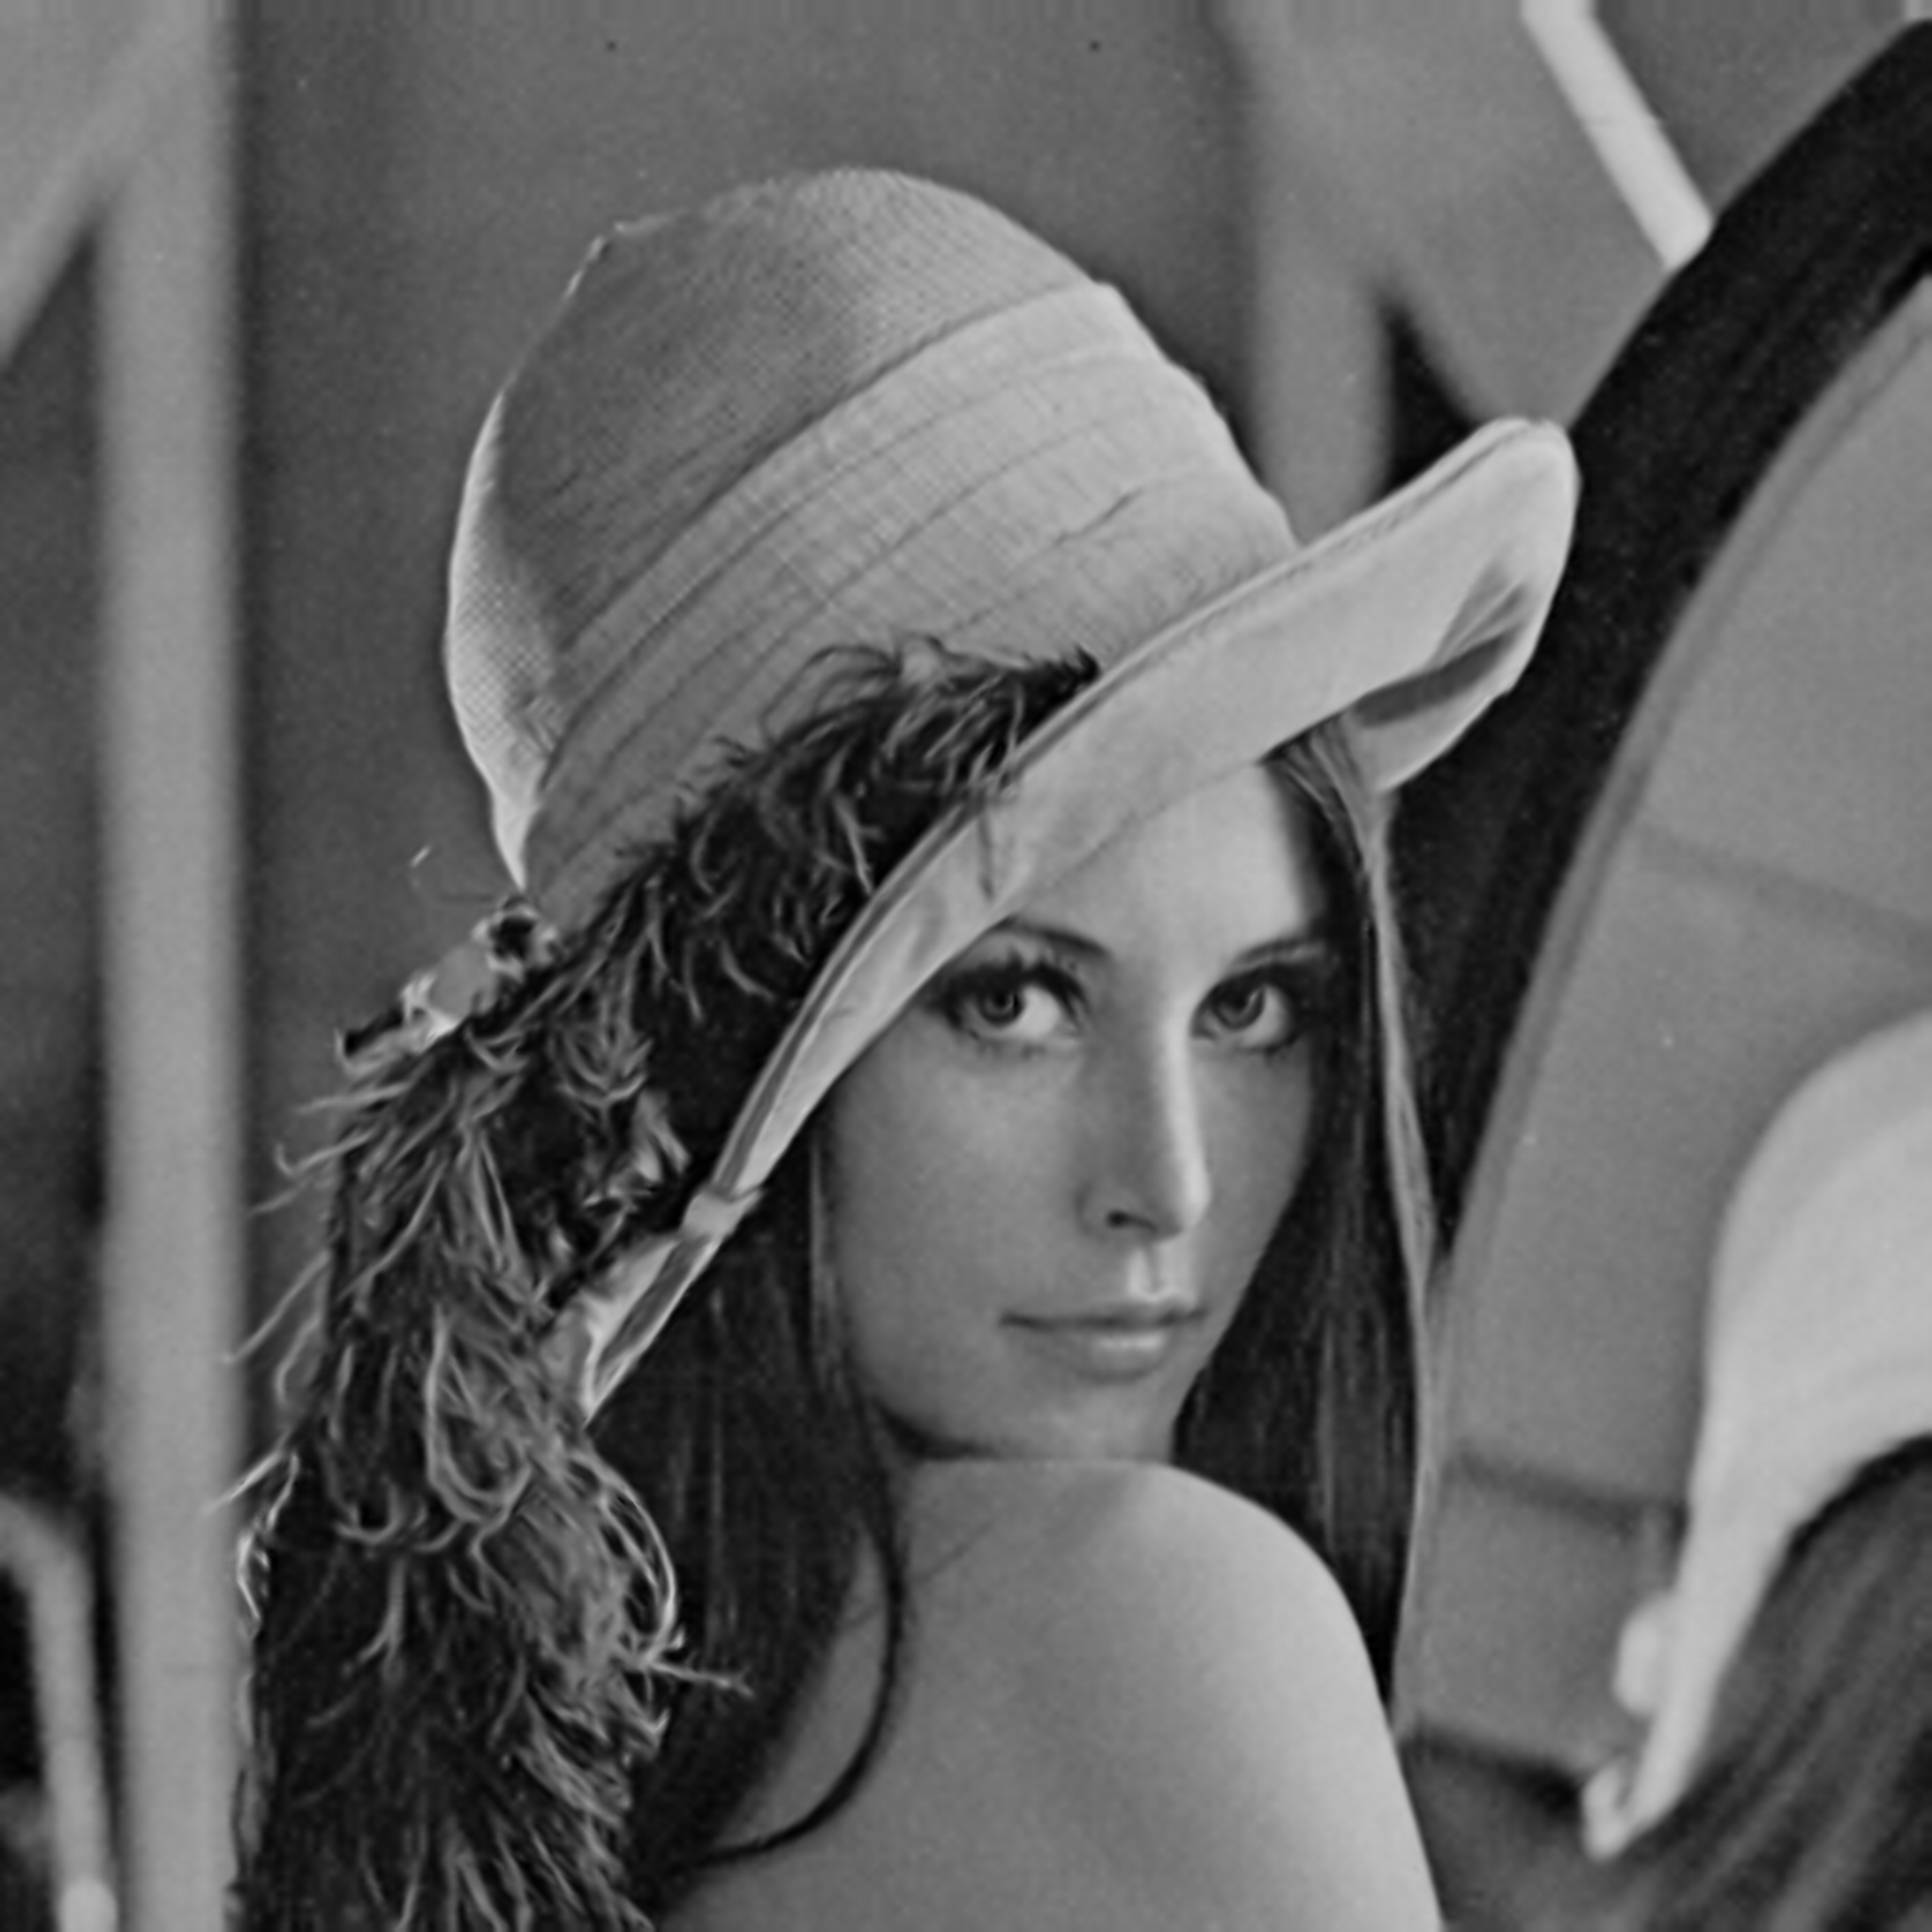
\includegraphics[width=7cm]{lena_normal.png}
\label{fig:subfig_a}
}
\subfigure[Imagem após a aplicação do filtro Sobel]{
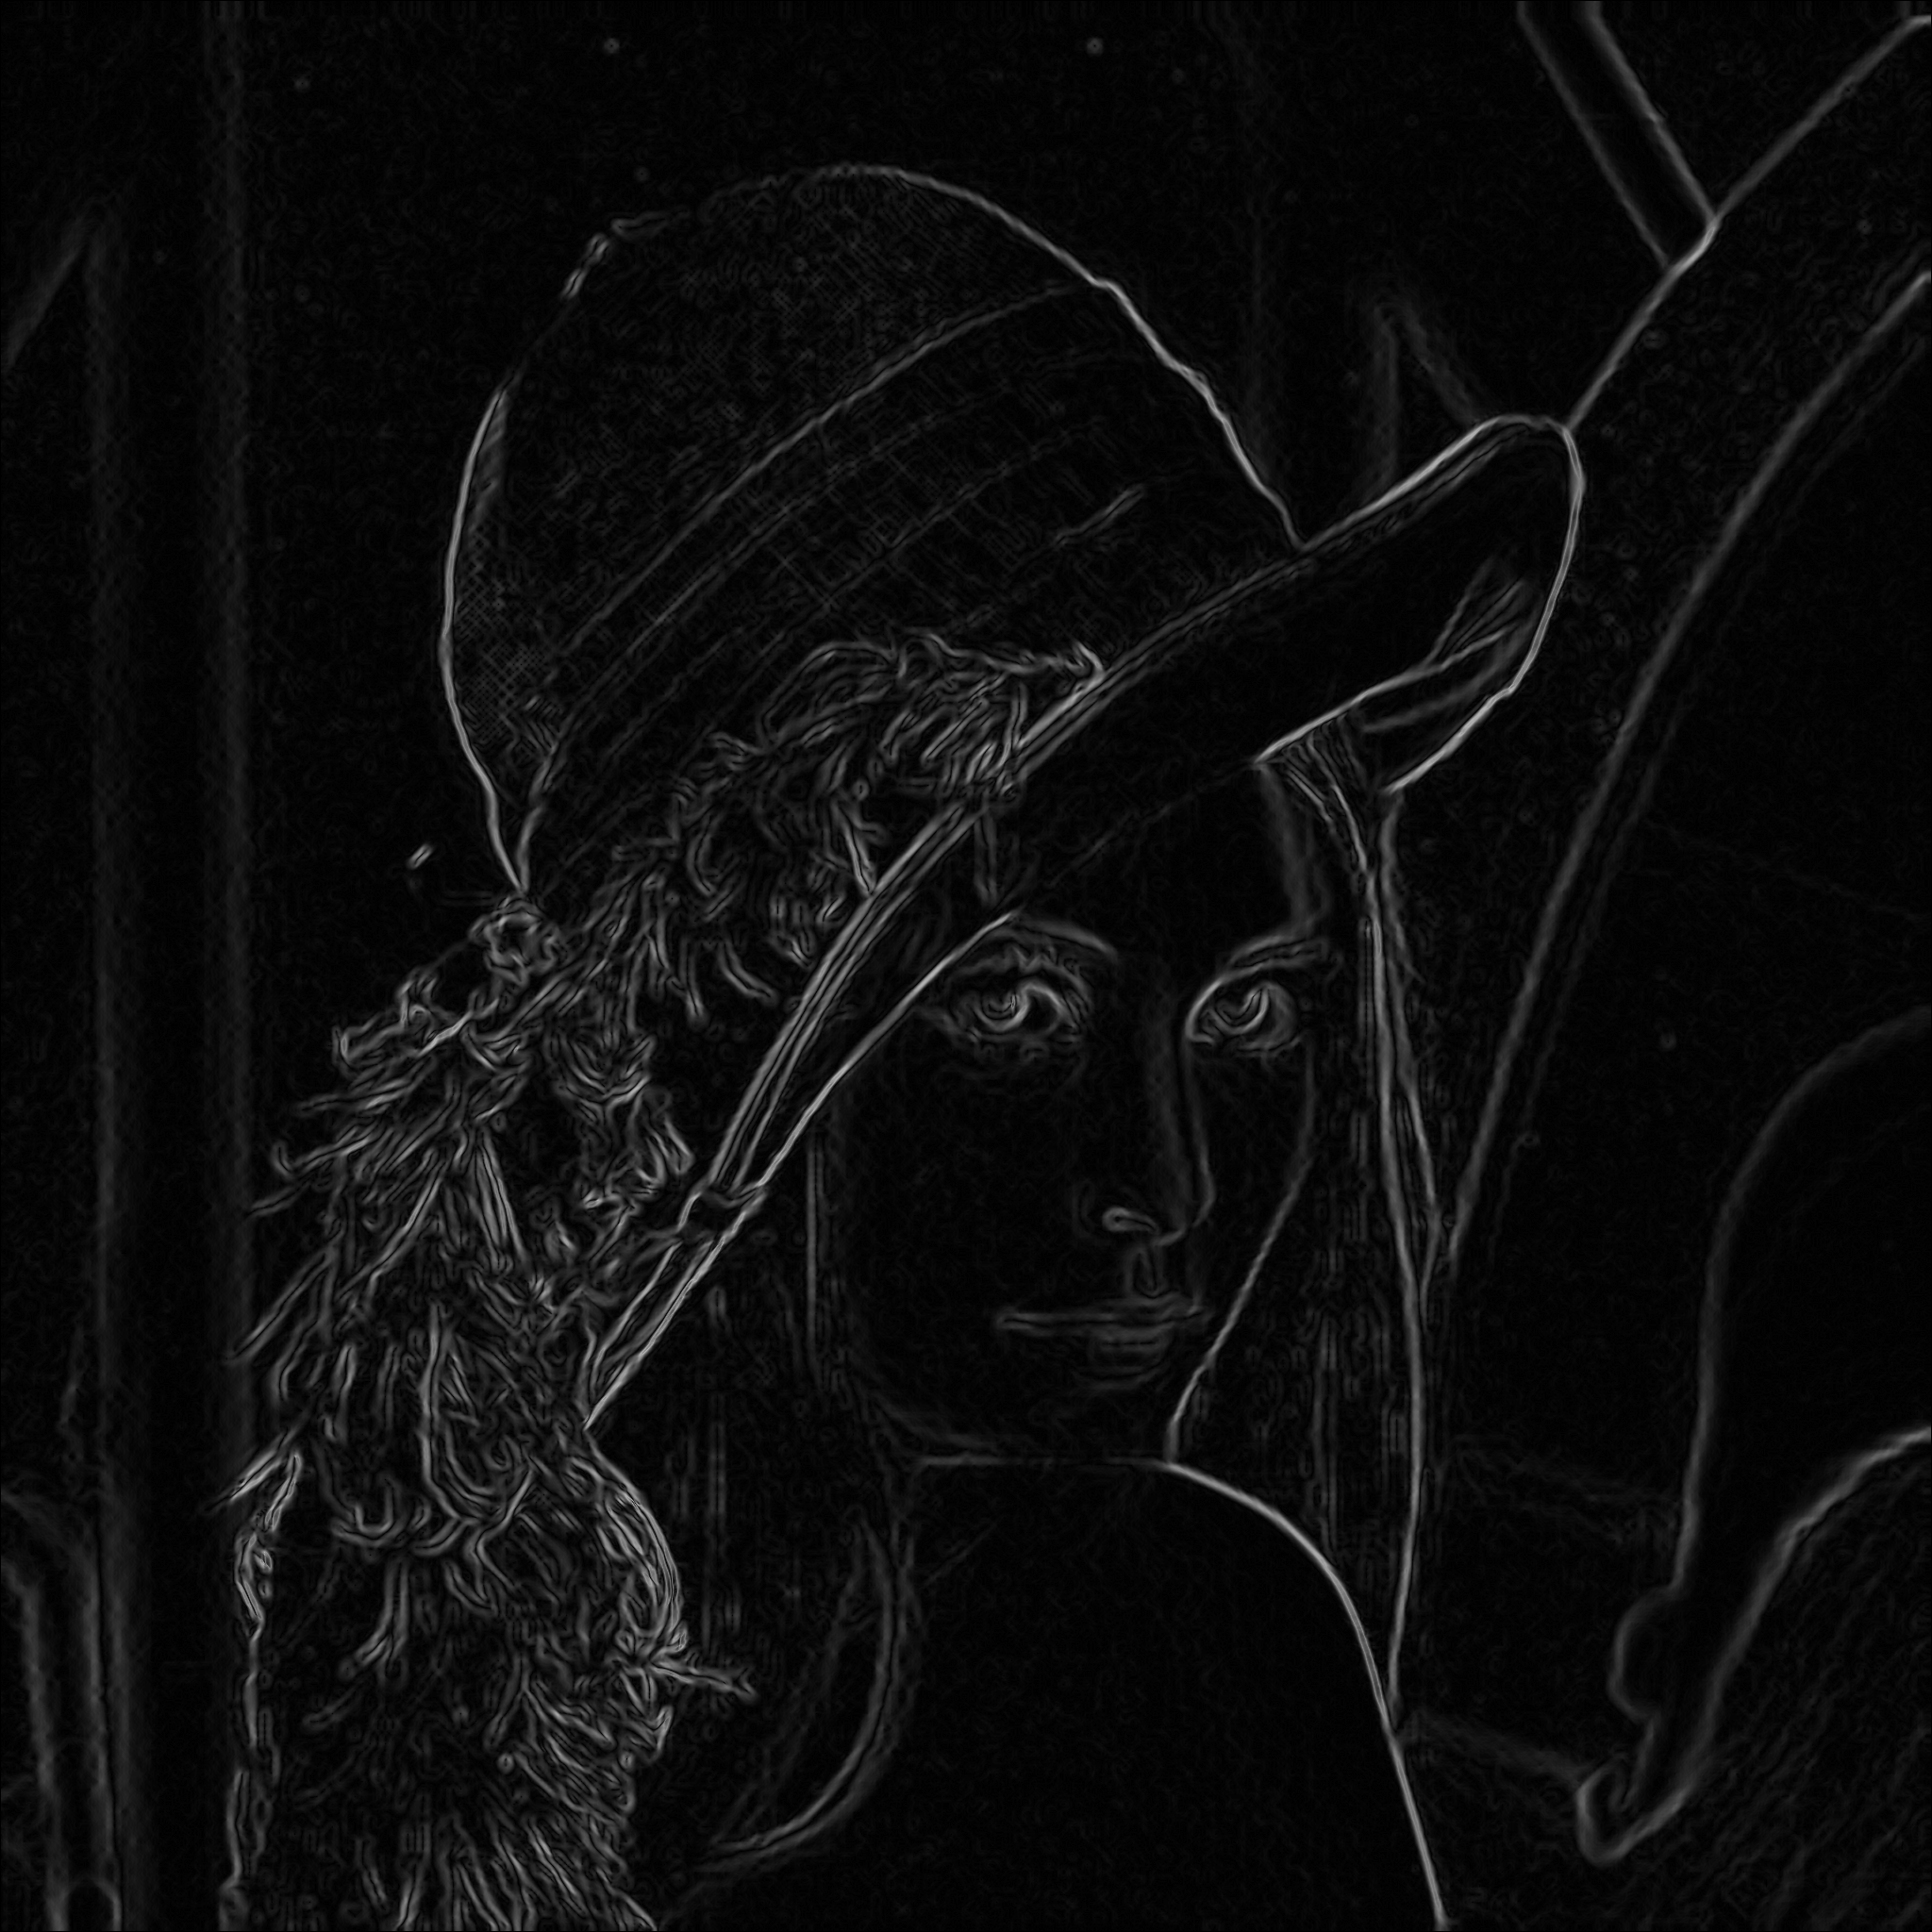
\includegraphics[width=7cm]{lena_sobel.png}
\label{fig:subfig_b}
}
\label{fig:sobel_filtro}
\caption{Resultado da aplicação filtro Sobel para detecção de borda}
\end{figure}

\FloatBarrier
\subsubsection{Tempo médio de execução}
O gráfico da Figura \ref{fig:sobel_tempo} apresenta os resultados obtidos dos tempos médios de execução da aplicação do Filtro Sobel em função das dimensões das imagens.
\FloatBarrier
\begin{figure}[!ht]
\centering
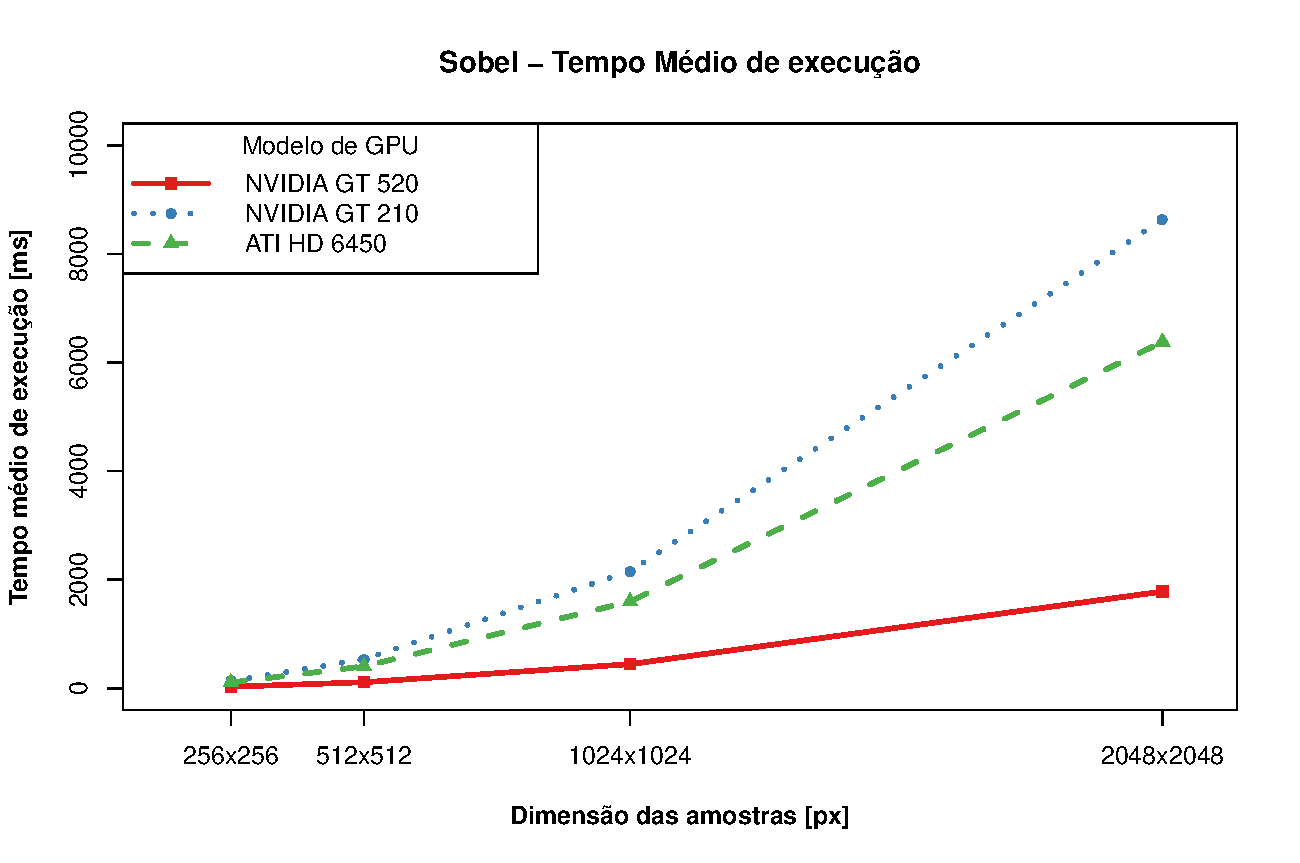
\includegraphics[width=0.9\textwidth]{sobel_tempo_medio_exec.pdf}
\caption{Sobel - Tempo médio de execução}
\label{fig:sobel_tempo}
\end{figure}
\FloatBarrier
A Nvidia Geforce GT 520 alcançou os menores tempos médios de execução e obteve o melhor desempenho. Seguido da ATI Radeon HD 6450 e da Nvidia Geforce 210.
\FloatBarrier
\subsubsection{Taxa média de transferência de dados da memória}
Os gráficos das Figuras \ref{fig:subfig_c} e \ref{fig:subfig_d} mostram que, apesar da Nvidia Geforce 210 ser da arquitetura Tesla, ela apresentou um desempenho muito próximo ao da Nvidia Geforce GT 520, que possui é da arquitetura Fermi ( sucessora da Tesla). A ATI Radeon HD 6450 foi a que teve as piores taxas de transferência, porém, é possível observar que, ao contrário das GPUs da Nvidia, as taxas de transferência da ATI Radeon HD 6450 foram aumentando a medida que o tamanho das imagens também aumentava. Isso sugere que \textbf{talvez o tamanho das amostras escolhidas não seja suficiente pra avaliar toda a capacidade dessa GPU}.
\FloatBarrier
\begin{figure}[!ht]
\centering
\subfigure[Taxa média de transferência do Host para o device]{
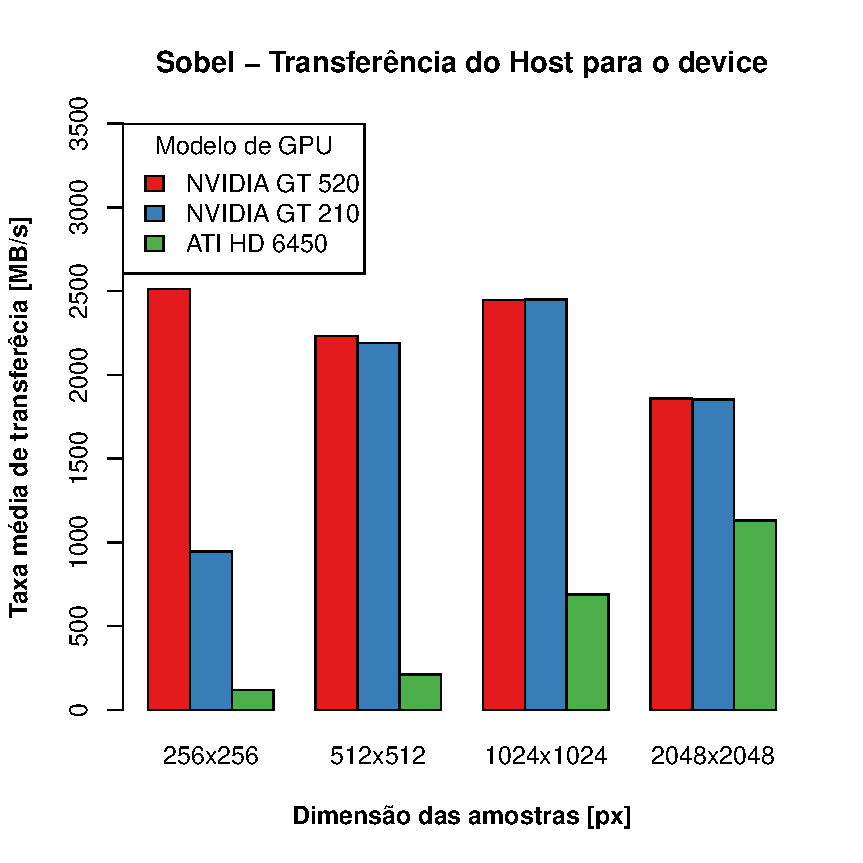
\includegraphics[width=7cm]{sobel_taxa_media_transfer_escrita.pdf}
\label{fig:subfig_c}
}
\centering
\subfigure[Taxa média de transferência do Device para o host]{
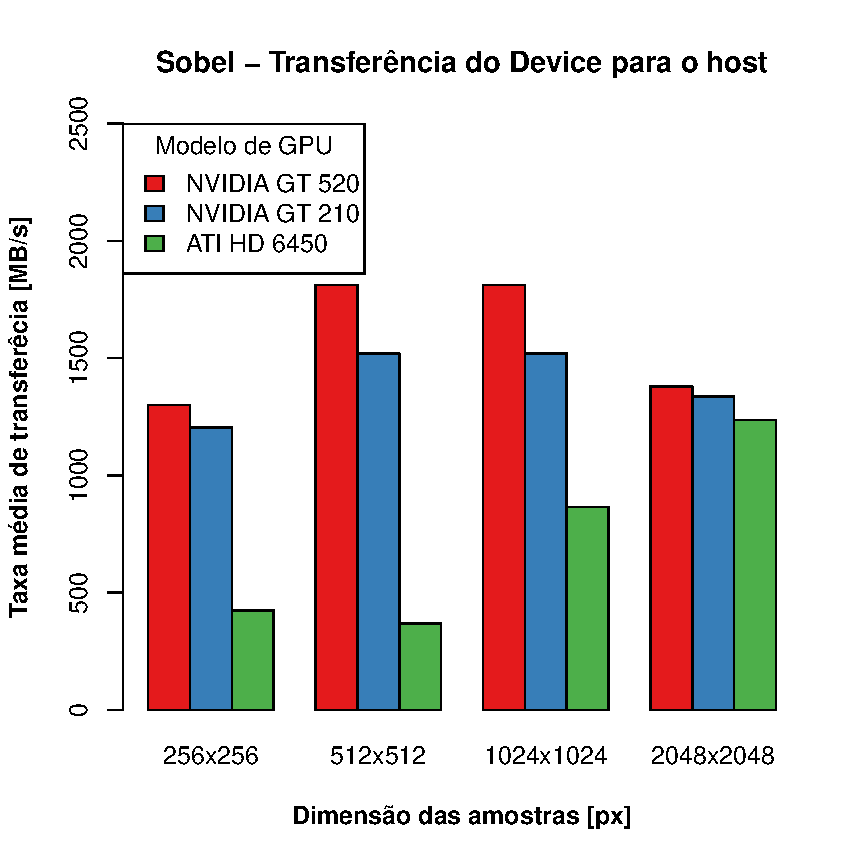
\includegraphics[width=7cm]{sobel_taxa_media_transfer_leitura.pdf}
\label{fig:subfig_d}
}
\label{fig:taxa_transfer}
\caption{Comparação do desempenho das taxas de transferência do filtro Sobel}
\end{figure}
\FloatBarrier

\FloatBarrier
\subsection{Filtro Passa-baixa}
Após aplicar o filtro Passa-baixa sobre as amostras, observamos, por meio da análise visual das imagens, que não existiu diferença nos resultados gerados pelas diferentes GPUs. Como esperado, ao se aplicar o filtro Passa-baixa sobre a imagem da Figura. \ref{fig:subfig_e} observamos na Figura \ref{fig:subfig_f} um aumento na luminosidade e a atenuação do contraste da imagem.     
\begin{figure}[!ht]
\centering
\subfigure[Imagem original]{
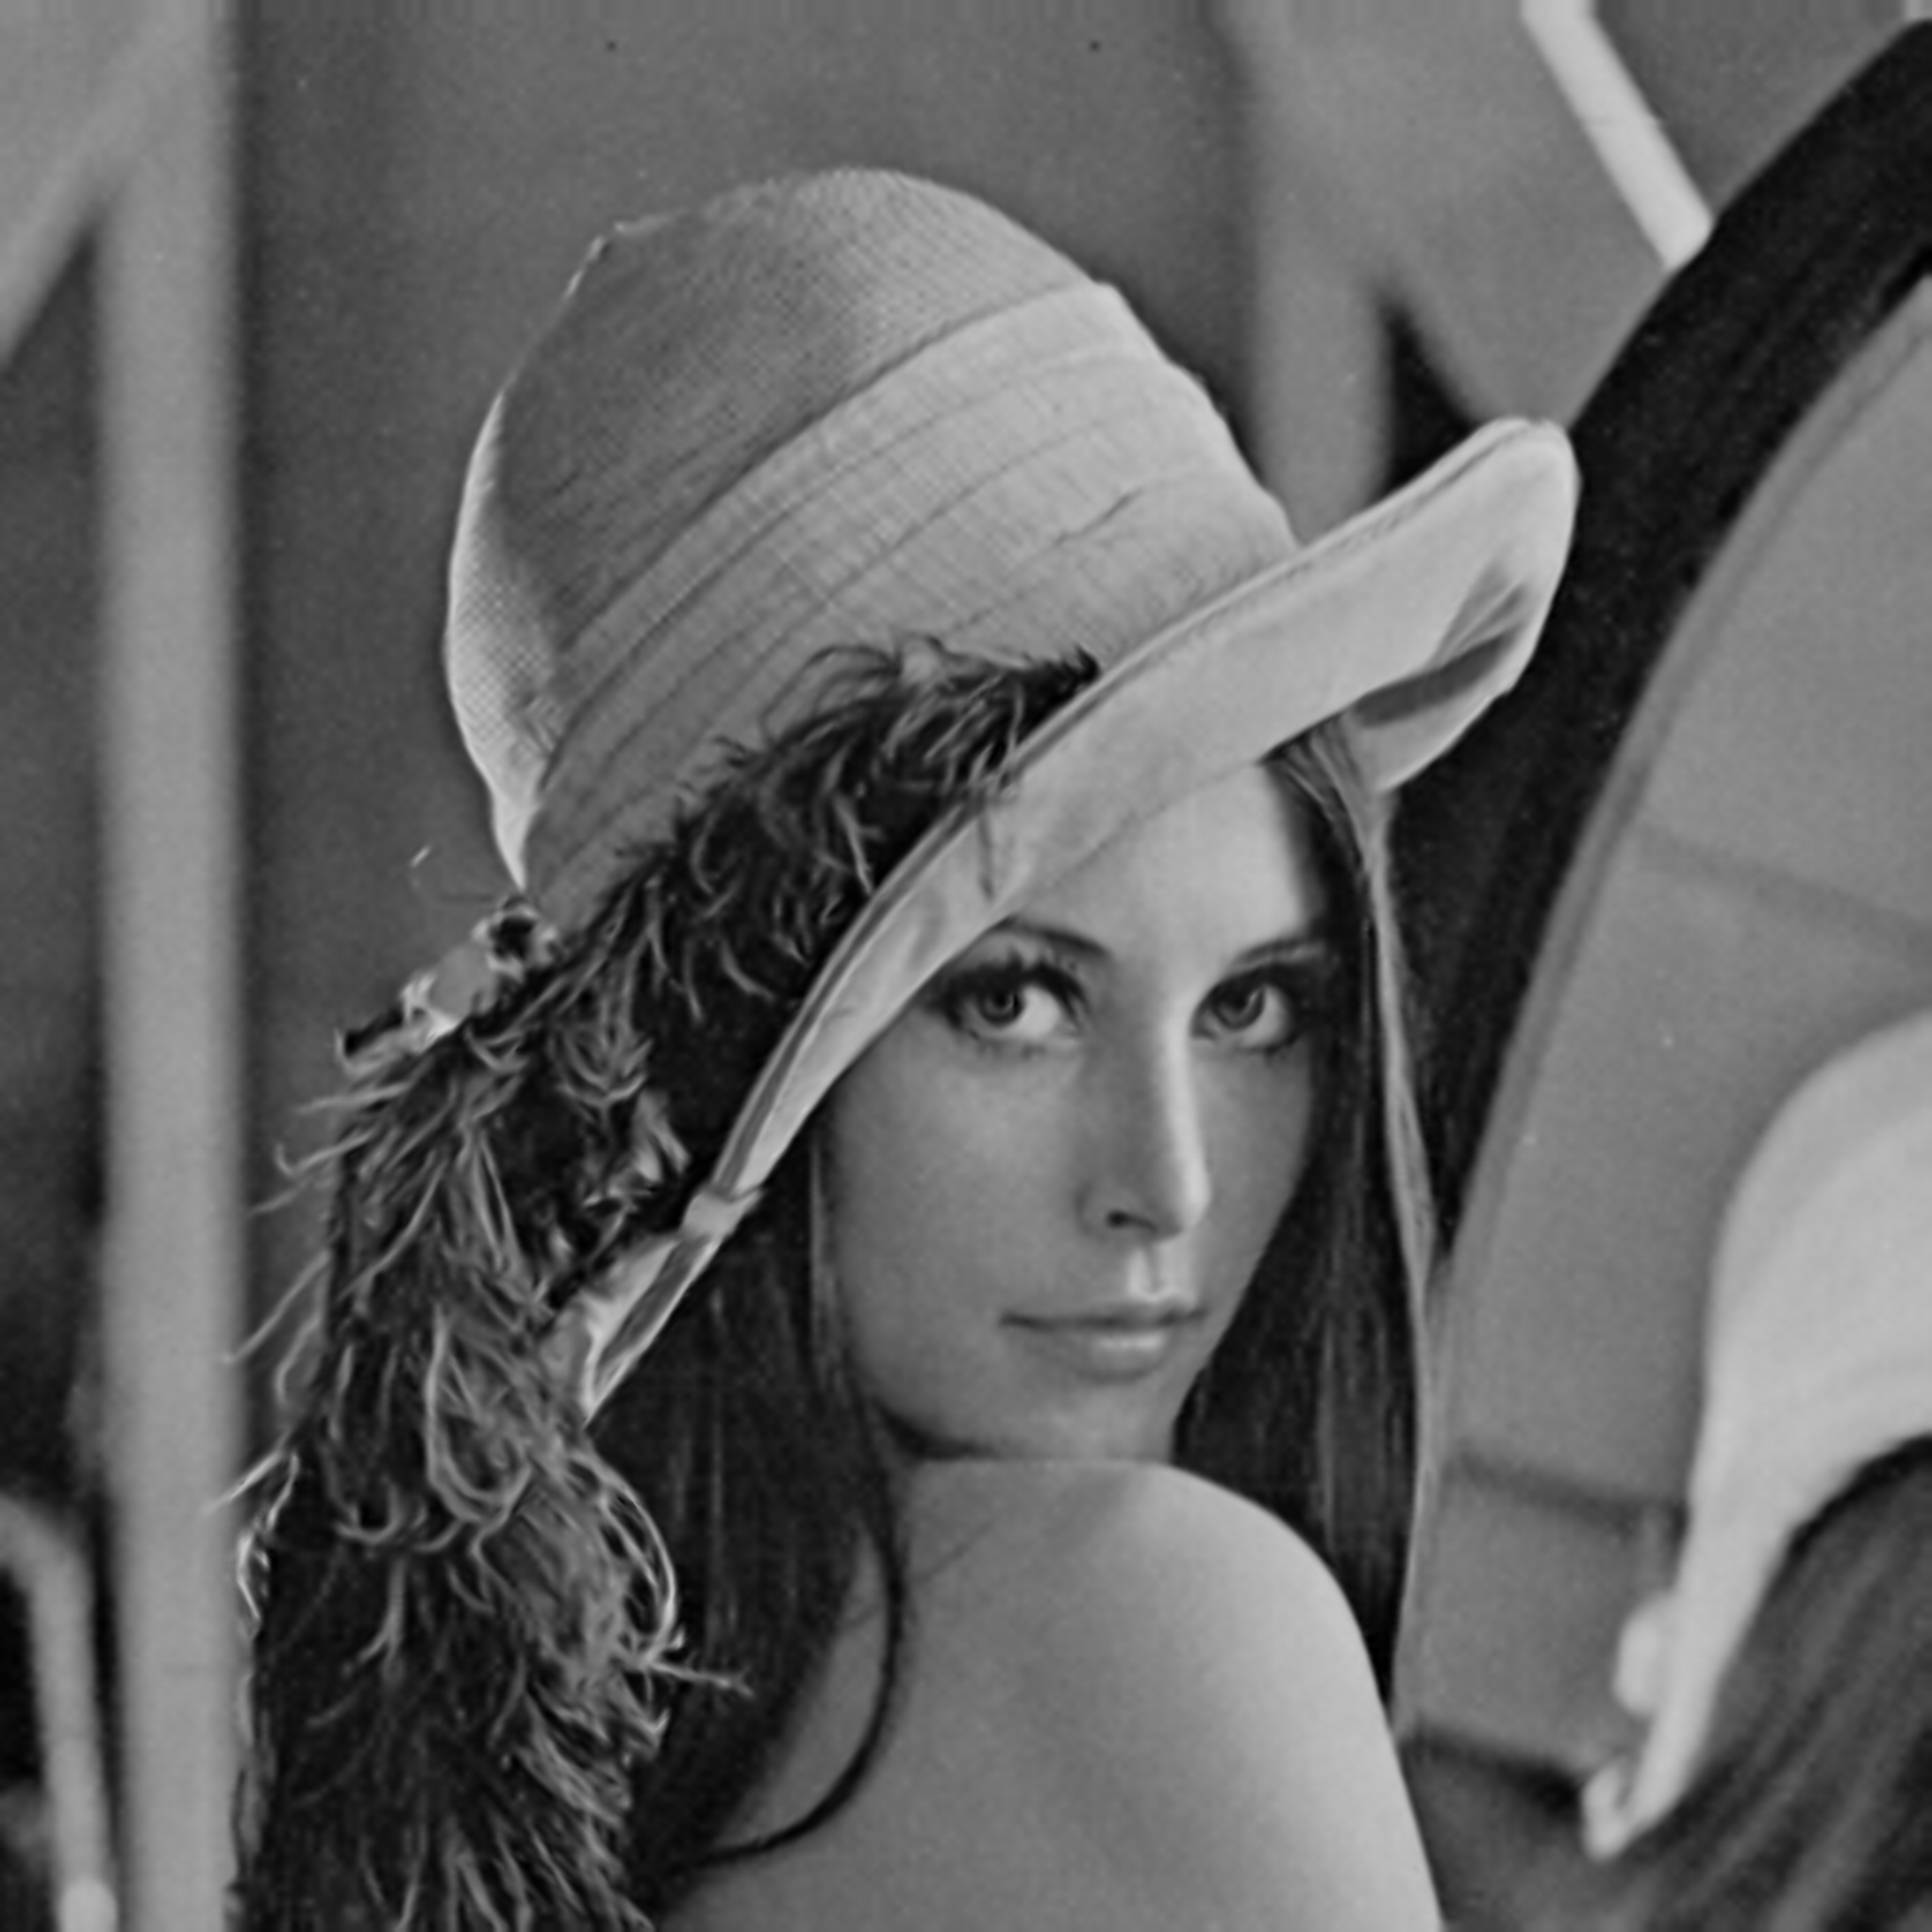
\includegraphics[width=7cm]{lena_normal.png}
\label{fig:subfig_e}
}
\subfigure[Imagem após a aplicação do filtro Passa-baixa]{
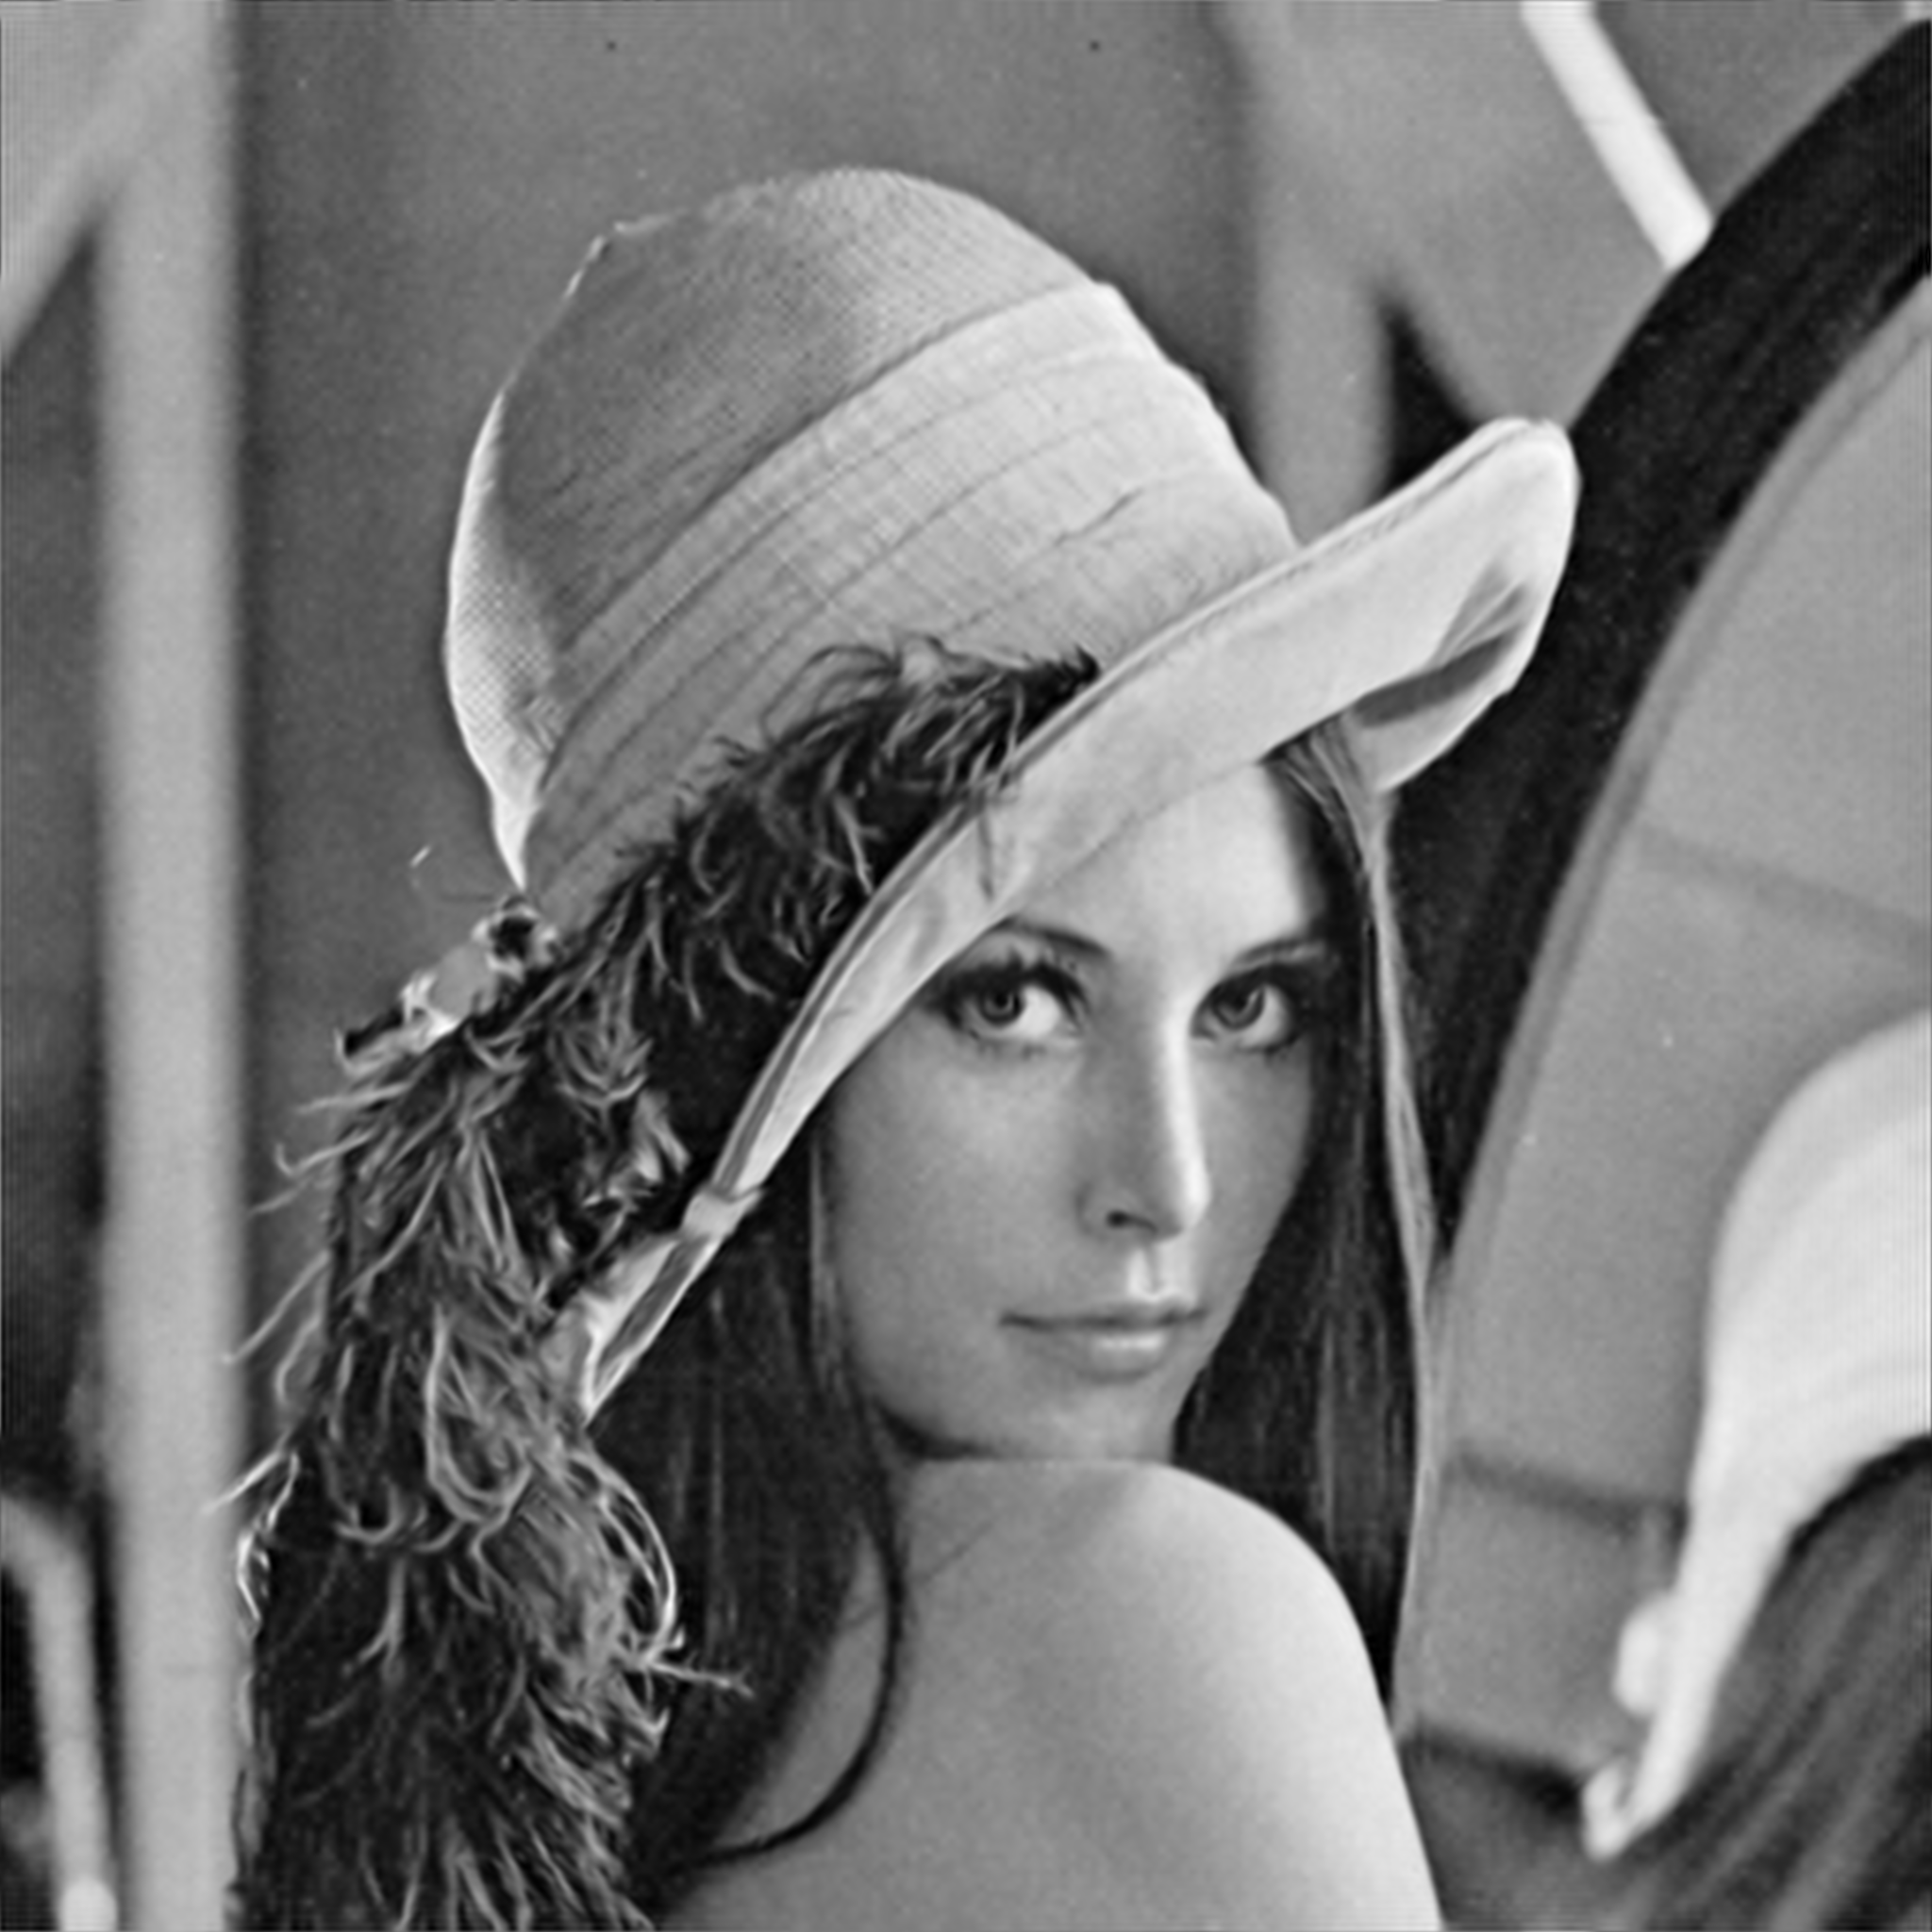
\includegraphics[width=7cm]{lena_passa_baixa.png}
\label{fig:subfig_f}
}
\label{fig:passa_baixa}
\caption{Resultado da aplicação do filtro Passa-baixa}
\end{figure}
\FloatBarrier
\subsubsection{Tempo Médio de Execução}
A Figura \ref{fig:passa_tempo} apresenta as curvas do tempo médio de execução para GPU utilizada neste trabalho. A Nvidia Geforce GT 520 obteve os melhores tempos médios de execução para o Filtro Passa-baixa. A ATI Radeon HD 6450 obteve o segundo melhor desempenho, seguido da Nvidia Geforce 210.  
\begin{figure}[!ht]
\centering
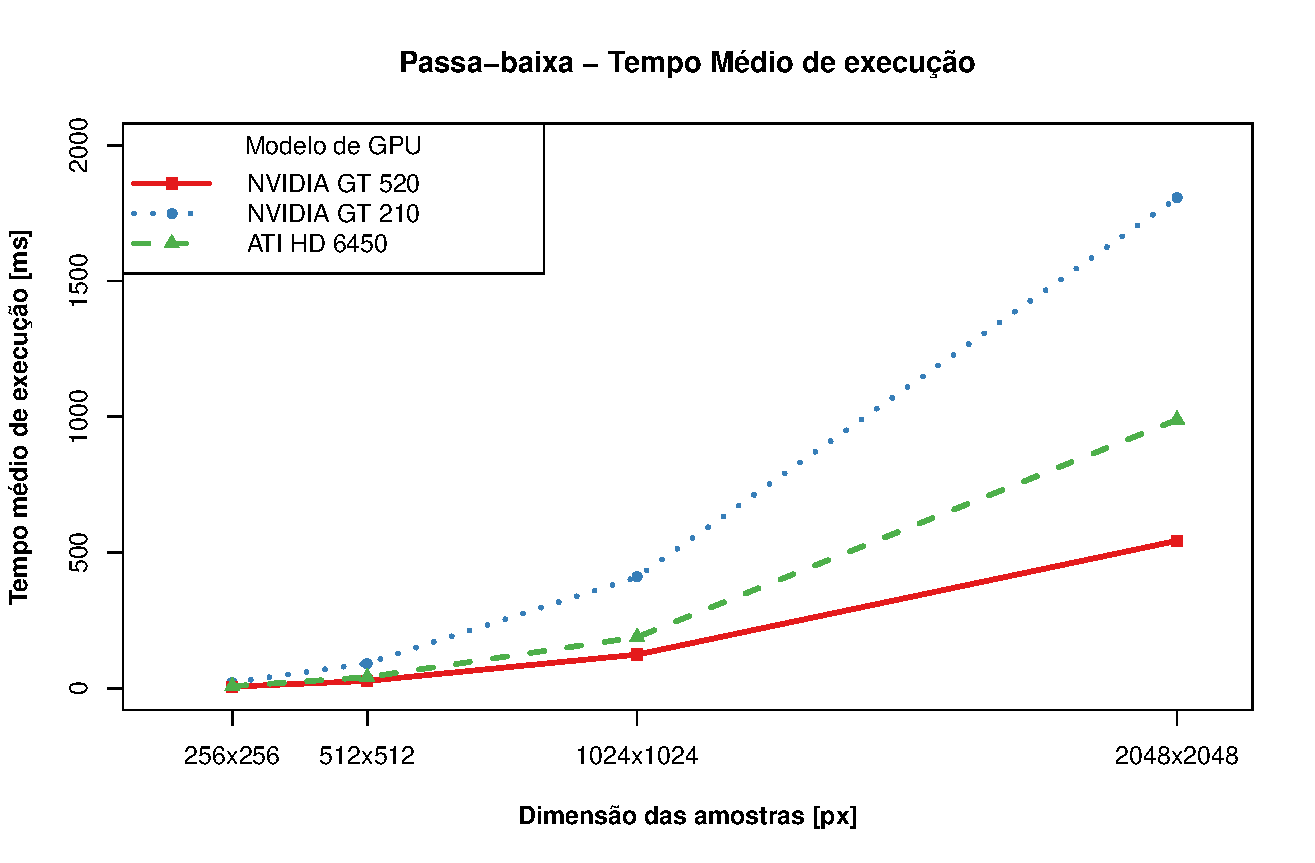
\includegraphics[width=0.9\textwidth]{fft_tempo_medio_exec.pdf}
\caption{Passa-Baixa - Tempo médio de execução}
\label{fig:passa_tempo}
\end{figure}
\FloatBarrier
\subsubsection{Taxa média de transferência de dados da memória}
Nas Figuras \ref{fig:subfig_g} e \ref{fig:subfig_h} é possível observar que as GPUs Nvidia mantiveram-se com as taxas médias de trasnferência muito próxmas novamente. A GPU da ATI apresentou, novamente, um crescimento das taxas de transfência táo maior fosse a entrada. Sendo que na Figura \ref{fig:subfig_h} observou-se que a GPU da ATI superou as GPUs da Nvidia para as amostras de tamanho 1024 e 2096. Esse comportamento que GPU ATI apresenta, possuem similiaridades com os resultados obtidos em \cite{ArchComp}, onde a GPU da ATI, obteve as melhores taxas somente para os maiores tamanhos das amostras.
\begin{figure}[!ht]
\centering
\subfigure[Taxa média de transferência do Host para o device]{
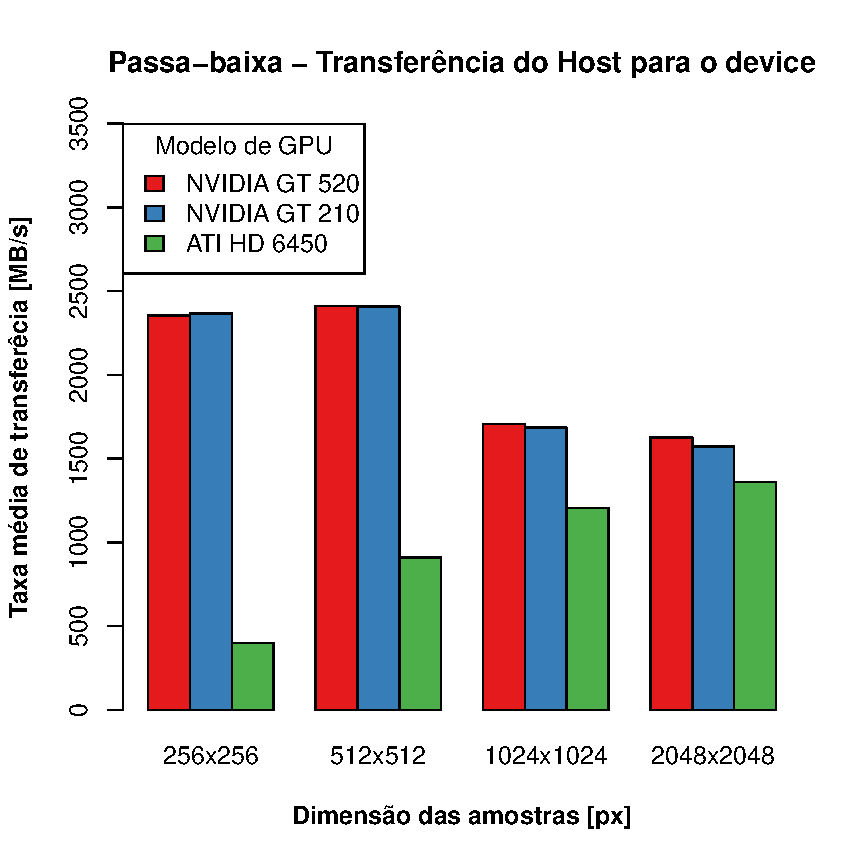
\includegraphics[width=7cm]{fft_taxa_media_transfer_escrita.pdf}
\label{fig:subfig_g}
}
\subfigure[Taxa média de transferência do Device para o host]{
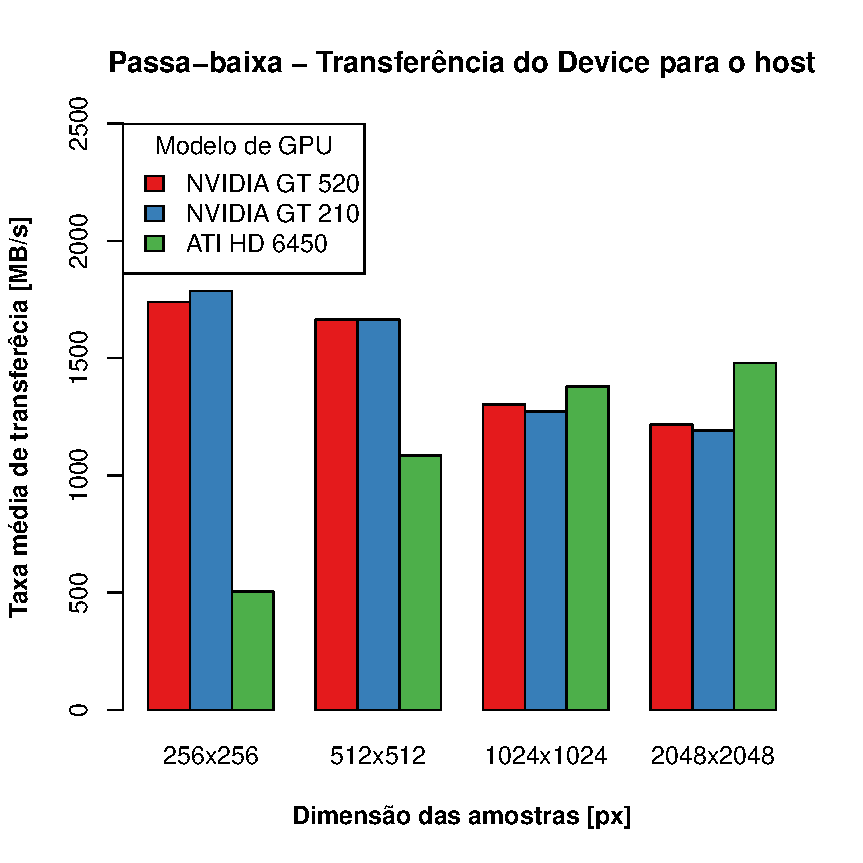
\includegraphics[width=7cm]{fft_taxa_media_transfer_leitura.pdf}
\label{fig:subfig_h}
}
\label{fig:subfiguras}
\caption{Comparação do desempenho das taxas de transferências do filtro Passa-baixa}
\end{figure}
\FloatBarrier
\bibliography{refs}
\bibliographystyle{plain}
\newpage
\appendix
\section{Códigos Fontes em OpenCL}
\subsection{Filtro Sobel}
Abaixo é apresentado o código fonte do \textit{kernel} do filtro Sobel, em OpenCL.
\lstinputlisting[language=C]{sobel_kernel.cl}
\newpage
\subsection{Filtro Passa-baixa}
Abaixo, é apresentado o \textit{kernel} do filtro passa baixa, em OpenCL.
\lstinputlisting[language=C]{passa_baixa.cl}

\end{document}
